%\documentclass[draft,landscape, 11pt, oneside]{report}
\documentclass[landscape, 11pt, oneside, twoside]{report}
\usepackage[a4paper, left=1cm, right=1cm, top=2.5cm]{geometry}
\usepackage{lmodern}
\usepackage{hyperref}
\usepackage{titlesec}
\usepackage{scrextend}
\usepackage{array}
\usepackage{ProphetPanel}
\usepackage{fontspec}
\usepackage[T1]{fontenc}
\usepackage{longtable}
\usepackage{ProphetTerms}
\usepackage{float}
\usepackage{setspace}
%\usepackage[inline]{showlabels}
\setmainfont[
 BoldFont={FiraSans-Bold}, 
 ItalicFont={FiraSans-Italic},
 ]{FiraSans}
\setlength{\parindent}{0pt}
\setlength{\parskip}{1em}
\setlength{\evensidemargin}{0cm}
\setlength{\oddsidemargin}{2cm}
\setlength{\paperheight}{210mm}
\setlength{\paperwidth}{297mm}
\setlength{\textwidth}{22cm}
\setlength{\footskip}{2.5cm}
%% globals
\newcommand{\version}{2.X}
\newcommand{\paramgeneral}[1]{\textbf{#1}}
\newcommand{\button}[1]{\textbf{#1}}
\newcommand{\patchparameter}[2]{\paramgeneral{#2 - #1}}

% additional patch parameters
\newcommand{\clockspeed}{\patchparameter{0}{Clock/Speed}}
\newcommand{\lfoshape}{\patchparameter{1}{LFO Shape}}
\newcommand{\lfotarget}{\patchparameter{11}{LFO Target}}
\newcommand{\lfosync}{\patchparameter{111}{LFO Sync}}
\newcommand{\vibspeed}{\patchparameter{2}{Vibrato Speed}}
\newcommand{\lforange}{\patchparameter{22}{LFO Frequency Range}}
\newcommand{\vibamt}{\patchparameter{3}{Vibrato Amount}}
\newcommand{\modwheelaction}{\patchparameter{33}{Modulation Wheel Action}}
\newcommand{\moddelay}{\patchparameter{4}{Modulation Delay}}
\newcommand{\modwheeltarget}{\patchparameter{44}{Modulation Wheel Target}}
\newcommand{\2ndenv}{\patchparameter{5}{2nd Envelope Shape}}
\newcommand{\filenv}{\patchparameter{55}{Filter Envelope Shape}}
\newcommand{\envrouting}{\patchparameter{555}{Envelope Routing}}
\newcommand{\bentarget}{\patchparameter{6}{Bender Target}}
\newcommand{\bendrange}{\patchparameter{66}{Bender Target}}
\newcommand{\glide}{\patchparameter{7}{Glide Time}}
\newcommand{\assignprio}{\patchparameter{77}{Assigner Priority}}
\newcommand{\detune}{\patchparameter{8}{Unison Detune Amount}}
\newcommand{\oscpitchmode}{\patchparameter{88}{Oscillator Pitch Mode}}
\newcommand{\spread}{\patchparameter{888}{Spread Amount}}
\newcommand{\ampvel}{\patchparameter{9}{Amplitude Velocity}}
\newcommand{\filvel}{\patchparameter{99}{Filter Velocity}}
\newcommand{\syncbug}{\patchparameter{999}{Sync Bug Switch}}


% buttons
\newcommand{\numberpad}[1]{\textbf{button #1}}
\newcommand{\totape}{\button{To Tape}}
\newcommand{\fromtape}{\button{From Tape}}
\newcommand{\tune}{\button{Tune}}
\newcommand{\preset}{\button{Preset}}
\newcommand{\record}{\button{Record}}
\newcommand{\seq1}{\button{Seq 1}}
\newcommand{\seq2}{\button{Seq 2}}
\newcommand{\arpud}{\button{Arp U/D}}
\newcommand{\arpass}{\button{Arp Assign}}

% panel controls
\newcommand{\polymodenv}{\patchparameter{Poly-Mod}{Envelope}}
\newcommand{\polymodosc}{\patchparameter{Poly-Mod}{Oscillator B}}
\newcommand{\polymodfreq}{\patchparameter{Poly-Mod}{Frequency Target}}
\newcommand{\polymodfilter}{\patchparameter{Poly-Mod}{Filter Target}}

\newenvironment{flowtext}{\addmargin[0cm]{0cm}}{\endaddmargin} % standard text width (reduced for layout)
\newcommand{\pp}[1]{} % patch parameter
\newcommand{\app}[2]{} % additional patch parameter, 1: number, 2: name


%%\title{[DRAFT] User Manual for the GliGli upgraded Prophet-600}
%%\pagestyle{myheadings}\markright{[DRAFT] User Manual for the GliGli upgraded Prophet-600}
%%\makeatletter
%%\renewcommand\chapter{\pagestyle{myheadings}\markright{[DRAFT] User Manual for the GliGli upgraded Prophet-600}\global\@topnum\z@\@afterindentfalse\secdef\@chapter\@schapter}
%%\makeatother
\titleformat{\chapter}[display]{\LARGE\bfseries}{}{0.0cm}{}
\titlespacing{\chapter}{0pt}{*0}{*0}
\titlespacing{\section}{0pt}{*0}{*0}


%%
%% Document Start
%%


\begin{document}

\raggedbottom
\singlespacing

\begin{titlepage}
\pagenumbering{gobble}

% this it the title "Prophet-600"
  \begin{tikzpicture}[scale=0.8]
    \begin{scope}[xslant=0.1]
        \SSGBit[1.5cm]{0,0}{12567}
        \SSGBit[1.5cm]{2.5cm,0}{57}
        \SSGBit[1.5cm]{5cm,0}{5734}
        \SSGBit[1.5cm]{7.5,0}{12567}
        \SSGBit[1.5cm]{10cm,0}{3567}
        \SSGBit[1.5cm]{12.5cm,0}{14567}
        \SSGBit[1.5cm]{15cm,0}{4567}
        \SSGBit[1.5cm]{17.5cm,0}{7}
        \SSGBit[1.5cm]{20cm,0}{134567}
        \SSGBit[1.5cm]{22.5cm,0}{123456}
        \SSGBit[1.5cm]{25cm,0}{123456}
      \end{scope}
  \end{tikzpicture}

  \vspace{1cm}
  
  
  \Huge
  User Manual \vspace{0.4cm} \\
  \Large
  Edition: version v2022 (RC1) (16.7.2022) \vspace{0.3cm}\\
  Firmware version: GliGli \version (RC1) by imogen\vspace{0.3cm}\\
  Editor / author: imogen / image-et-son 
  \normalsize

\end{titlepage}


\pagebreak
\pagebreak

%\maketitle
\tableofcontents


\pagestyle{myheadings}\markright{(DRAFT) Prophet-600 \version User Manual }
\makeatletter
\renewcommand\chapter{\pagestyle{myheadings}\markright{(DRAFT) Prophet-600 \version User Manual}\global\@topnum\z@\@afterindentfalse\secdef\@chapter\@schapter}
\makeatother

\pagebreak
\chapter{Introduction to the GliGli Prophet-600 Firmware Upgrade}

\pagenumbering{arabic}
\setcounter{page}{1}

\begin{flowtext}

The original Sequential Circuits Prophet-600 from around 1982 is run by a Zilog Z80 processor. This processor (and the firmware written for it) is pushed beyond its limits for computing and applying the voltages, for scanning user inputs and managing MIDI events. The necessary compromises made the instrument steppy, glitchy and non-responsive. That is a pity, because the basic synth voice hardware of the Prophet-600 is good: unlike DCO synths which became popular and affordable at the time, the Prophet-600 is a 6 voice analog synthesizer driven by 2 voltage controlled oscillators (VCOs) and a 24db low pass filter per voice, all implemented using the renowned Curtis chips \cite{curtis}. The hardware also provides hard sync, frequency modulation and even modulation of cut-off by VCO. It is very versatile. The shortcomings of the original Prophet-600 were due only to the unfortunate circumstance that the selected and commonly available micro-processors at the time were not powerful enough for the Prophet-600. So the idea to make use of a more modern processor 30 years later was interesting. Around 2013 GliGli \cite{gligli} started reverse engineering the original firmware for the Z80 and found that the Z80 can be replaced by a (more) modern Teensy++ 2.0 USB programmable microprocessor \cite{teensy} (with some hardware modifications). This was the start of what is now know as the \textit{Prophet-600 GliGli firmware upgrade}. GliGli describes his motivation as follows:

\begin{addmargin}[2cm]{1cm}

\textit{I love vintage analog synthesizers, and to be honest, my dream synth would be a Prophet-5, but when I heard what the Prophet-600 was capable of tone wise, I immediately thought its major weaknesses -- the lousy computer part, software envelopes and LFO -- could become its strength with a remake; basically the whole internal synth in voltage-controlled from a nice 14bit DAC, so with a fast modern micro controller, it could become awesome, maybe even better than a Prophet-5!}

\end{addmargin}

There are various modifications and modern CPU "implants" for some vintage analog synthesizers. Since the Teensy++ 2.0 board fits in to the same 2x20 pin standard socket of the Z80, the decisive advantage of the GliGli approach is that it is an easy-to-install and non-destructive firmware drop-in replacement\footnote{There are two versions of the Prophet-600. One has the Z80 on a socket. In this case replacement is truly "drop-in". The other version has the Z80 soldered to the circuit board. In this case the Z80 needs to be removed and a socket has to be soldered in its place first.}. It is completely safe to try out the Teensy++ 2.0 upgrade because one can always remove the board and restore the Z80 without technical expertise or training. 

The Teensy++ 2.0 offers completely new possibilities. Just looking at specs: the Z80 version of the Prophet-600 ran at 4 MHz while the ATMEL processor on the Teensy board is operated at 16 MHz. Also, the on-board flash memory provides much better storage and firmware handling possibilities compared to the EPROM which the Z80 uses. The firmware does not rely on a battery for keeping patch data in memory. With the replacement the obvious limitations of the original Prophet-600 could be overcome - but more than that, it opened the possibility for new and for enhanced features. 

Developing the software was a major effort with low-level functions and basic hardware communication at the core, e.g. instruction to set voltages to the electronic components, MIDI (interrupt) implementation, multiplexer operations and DAC operations. On top of this there is the "musical" part of coding such as envelopes, LFOs, modulations and sequencing functions as well as UI functions. Many people have contributed, most probably out of curiosity and passion for synthesizers and driven by the excitement that such a project could not only be conjured up but also be implemented and brought to life. 

The first stable version of the firmware upgrade was version 2.0 in 2014. An intermediate release (or at least something close to a release) version 2.1 Release Candidate 3 (2.1 RC3) has been available from September 5th 2015 on GliGli's webpages \cite{gligli}. The latest release version \version is the result of continued development between September 2021 and March 2022. It is meant as a celebration and revival of the original idea and it provides various new features and also significant improvements in core functions. The latest firmware version can be found on the project page\cite{newversion}.

While there is a realistic backlog of additional ideas to come in the future, there is a clear end of Prophet-600 upgrade story in sight because of ultimate hardware limitations. Firstly, PJRC (the manufacturer of the Teensy boards) has stopped producing the Teensy++ 2.0 board, so that it has become difficult to find them. Secondly, after extensive performance testing in the latest firmware developments efforts, it has become clear that the performance (smoothness and responsiveness of controls, timely and accurate processing of information) is finally limited by the built-in hardware, in particular the DAC (limited by voltage rise times) and multiplexer (limited by switching times). 

If you own a Teensy++ 2.0 upgraded Prophet-600 you can still enjoy some exciting new developments. The following is a compact summary of the improved and the new features. The manual generally refers to the latest version \version. Differences between versions are marked or commented in the text for your information. Share the passion for analog synthesizers with the Prophet-600 upgrade story!  

\begin{flushright}
  \textit{imogen / image-et-son}
\end{flushright}

\pagebreak
\section{What you can expect from the Firmware Upgrade}

\textbf{General features compared to the original Z80 version}
  
\begin{itemize}
  \setlength\itemsep{0cm}
  \item Greater resolution of many of the sound parameters with an improved refresh rate that makes the instrument much more responsive, again improved in \version using a dynamic scheme for reading user controls.
  \item Faster and smoother ADSR envelopes with support for two speed regimes (slow, fast) and two shapes (linear, exponential). The latest version \version has new linear shapes which were inspired by Prophet-5 rev 1/2 envelopes and designed to be more organic and musical than the former linear shapes.
  \item Positive and negative envelope amount settings for filter and poly-mod 
  \item A new LFO function generator with a wider frequency range from one cycle every 20 seconds to about 60Hz
  \item Assignable, random and up/down arpeggiator, optionally sync-able to external MIDI and analog clock
  \item Multiple note assignment modes including last/low/high note priority
  \item Full MIDI In control including amplitude and filter velocity sensitivity with an external keyboard controller, continuous controllers (CC) of all sound parameters, program change (PC) to choose current preset
  \item A dedicated vibrato which can be controlled by the modulation wheel
  \item Unison chord mode
  \item Four new LFO waveforms in addition to the original triangle and square including sine, random stepped, noise (like on the original Prophet-5, but non-periodic) and sawtooth (ramp up)
  \item Mix overdrive which now allows the output from both oscillators to drive the mix VCAs A and B harder as well as the Curtis 4 pole filter resulting in new sonic possibilities
  \item Pitch Wheel interval selection of plus/minus one octave, a whole tone, a minor third and a fifth
  \item Pitch Wheel reassignment to the VCF and Volume or off   
  \item Modulation wheel intensity setting in four steps, with a smooth (exponential) action in the latest version \version
  \item A new and improved tuning procedure
  \item Octave, chromatic and free oscillator course pitch control, with different options for oscillators A and B in the latest version \version
  \item Debounce feature that prevents unintended re-triggering caused by the old keyboard
\end{itemize}

\textbf{Specific features from version 2.1 RC3 onwards}
  
\begin{itemize}
  \setlength\itemsep{0cm}
  \item Polyphonic step sequencer
  \item Per note tuning
  \item Improved UI, introducing display of -50...50 range for bipolar dials and center deadband for better handling  
  \item VCF limit option
  \item Maintenance mode / adjustment scaling
  \item Vintage (spread) function for voice variations in tune and envelopes, re-designed as a continuous parameter in version \version which can even be controlled by MIDI CC   
  \item Support for pedal to sustain notes and to hold chords (in unison)
  \item On-the-fly transpose function for arpeggiator and sequencer
\end{itemize}

\textbf{Features with version \version}
  
\begin{itemize}
  \setlength\itemsep{0cm}
  \item Smoother and more responsive actions of all controls due to dynamic scanning scheme 
  \item Softer (exponential) action of LFO control (frequency and amount) to provide more travel for common "musical" value ranges
  \item Super accurate oscillator B fine tuning using a slow mid region
  \item Improved envelope shapes inspired by the Prophet-5 rev 1/2 shapes, replacing the linear shape in versions 2.0 and 2.1 RC3.  
  \item Revised and more intuitive organisation of menu parameters in groups with corresponding "cheat sheet"
  \item A new UI concept with pick-me-up behaviour, in order to avoid discontinuous value changes and to make the differences between panel and internal values transparent 
  \item Switchable panel layout with choices: Mix / Glide (Sequential Circuits / SCI layout)and Volume A / Volume B (synthgraphics suported GliGli layout) 
  \item Flexible envelope routing allowing the poly-mod to be modulated by either envelope generator
  \item Ability to sync the LFO to the arpeggiator and sequencer
  \item Better MIDI integration possibilities through new local off mode and MIDI input into sequencer and arpeggiator
  \item Improved and protected patch management via MIDI, supporting single patch dump and loading MIDI patch to active controls 
  \item Changed arpeggiator patterns: omitting the top and bottom note repeat in the U/D arpeggiator pattern and removing note repeats in the random pattern
  \item Support for adjusting the external CV input amount
  \item Vibrato target VCA
\end{itemize}

In addition to this, several more technical / advanced changes were made such as the option to switch between "round robin" and "first" voice assign logic, the ability toggle a pulse width sync bug which has been introduced in the version 2.0 (and kept for compatibility in version 2.1 RC3), changes to remove the interference  of internal and external (MIDI) pitch bend by adding the two (as in the original SCI firmware), stabilization of the external analog clock input.

\section{On compatibility for those upgrading from 2.0 and 2.1 RC3}

You can upgrade the firmware by SysEx or by directly loading the firmware onto the Teensy++ 2.0 board via USB (see section \ref{fwupgrade}). When upgrading by SysEx, both patch data and settings are preserved. Backward compatibility is ensured, i.e. patches created in prior firmware version (including Z80) still work properly on new firmware versions. Note that as a general principle, before performing any upgrade the safekeeping of patches is not only best practice but also strongly recommended. The following contains some remarks which are relevant if you are upgrading to version \version from version 2.0 or 2.1 RC3.

\textbf{Panel}: If you have a synthgraphics overlay, there are some minor changes (also reflected in the figures in this manual). Firstly, the layout of the menu parameters has been changed - these are now grouped in themes and since there are more parameters, selecting a parameter requires three presses in some cases. So the "cheat sheet" that some users have attached to the left of the number pad is not correct any more. Secondly (and less significant), what was formerly the "amplitude envelope" is now referred to more generally as the "2nd envelope". There are additional envelope routing options so that this envelope has a more generalized role. 

\textbf{Vintage / Spread}: With 2.1 RC3 a "spread" switch was introduced as part of the global settings (not part of the patch). With version \version this has been removed from the settings and has been reintroduced as the patch parameter \textit{vintage spread}. It serves the same purpose, but it can be controlled continuously and it is more randomized than the former spread switch for more realistic results.

\textbf{Detune}: The unison detune has undergone a scaling re-design in version \version: the detune is now less pronounced at higher frequencies. This has been done to achieve the same subjective detuning effect across the whole frequency range. This is a change to the sound of the instrument and depending on how you use detune, your detuned unison patches may sound slightly different at higher registers compared to prior firmware versions. The idea is of course, that this is an agreeable change for everybody.

\textbf{Arpeggiator}: The arpeggiator patterns up/down and random have been changed in version \version

\textbf{MIDI CC}: Due to the change in menu parameters (obsolete parameters) and subsequent reshuffling (re-designation of the CC values for the legacy LFO frequency range), the specification of MIDI CC has changed slightly. As a result of rescaling of parameters the MIDI CC value to action has changed for LFO and vibrato frequencies and LFO and vibrato amounts as well as decay and release times of envelopes with linear shape. When loading older patches, the changes are taken into account to ensure compatibility.

\textbf{Envelopes}: The linear envelope shape has been revised in version \version. It is now a linear shape with an exponential tail (i.e. a softer roll-off) for decay and release. It was a deliberate decision to replace the linear shape altogether. Note that the smooth roll-off required a rescaling of the envelope decay and release controls for linear shapes. When loading older patches, the changes are taken into account to ensure compatibility: the effective decay and release times are preserved. However, the application of MIDI CC values is different, so if you are controlling sound by MIDI CC you may need to make adjustments.

\section{Credits and license}

The firmware upgrade project is an open source project. The GliGli code base (up to and including version 2.1 RC3) can be found in \cite{gligli} and the new code base of the latest development can be found in \cite{imogen}. When I first drafted this manual I hoped to put together a credits section by assembling a fair and comprehensive list of contributors. I have given up. There was no one who could, with authority, list and assess what came from where and who added what. From my research I can say that a \textbf{lot} of people have contributed and some have obviously spent considerable time to make this software as useful and consistent as possible. 

Let me just give you some highlights and a brief roundup. First, I think that the original 77 page technical documentation of the Prophet-600 by Stanley Jungleib \cite{p600siservicemanual} is great and such  documentation is both helpful and more than one can expect. Then there is an elaborate blog "Prophet-600 Spirit" by \textit{minisystem} \cite{p600spirit} which is legacy by now but still available. It contains a lot more technical information, Prophet-600 hardware related ground work, I would call it. I had the impression that it also helped the project. The contributors to the actual code can be obtained from the submit history of the code base on Github \cite{imogen}. Apart from GliGli (obviously) I found \textit{snickell} and \textit{Ricard Wanderlof} with many commits, although I haven't taken the time to disseminate their contributions in detail. Then there is the community, especially (but certainly not exclusively) on Gearspace (a common community platform for people to discuss music gear, not so long ago also known as Gearslutz): testing, giving feedback, spreading the word, supporting the project by appreciation and enthusiasm. Since I started picking up the development in November 2021 I joined up with a group of supporters and musicians loosely bound together by a forum thread on Gearspace. A number of active users have been especially helpful in prioritizing features, testing and proof reading. I neither want to list all of them, nor single someone out. Let me just say that developing the new envelopes and experimenting with different and sometimes really tricky aspects of the Prophet-600 hardware (e.g. multiplexers) would have been a lot less fun (and in parts even impossible) without an active community and dedicated co-workers.  

This user manual contains some texts and snippets written by other people. I compiled, merged, extended and in some case corrected the available information to an extent that makes it near impossible to trace everything back to its origins, let alone put in proper references. I just assume that all consent to the usage of their words. The overwhelming part of the text and the graphics are new.

The firmware  is under GPL v3 license, except files / libraries / other open source components that have their own license in the header. The usage of the software and related documentation (including descriptions and references to descriptions for making modifications to hardware) are understood to be at the user's own risk. The firmware program is distributed in the hope that it will be useful, but WITHOUT ANY WARRANTY; without even the implied warranty of MERCHANTABILITY or FITNESS FOR A PARTICULAR PURPOSE. See the GNU General Public License for more details.

\end{flowtext}

\pagebreak

\chapter{Finding your way around your new  Prophet-600}    

\begin{flowtext}

The different controls and interfaces of the Prophet-600 are shown schematically below. Throughout the document the corresponding nomenclature is used. In the original GliGli firmware upgrade the dials for oscillator A vs. B mix had been replaced by separate dials for oscillator A volume and oscillator B volume, at the expense of demoting the glide amount to a menu parameter. In the newest firmware version you have the choice to either use the \textit{GliGli} layout or the original \textit{Sequential Circuits (SCI)} layout. For more details on how to change the panel and on the parameters in each case see section \ref{panelswitch}.

\begin{samepage}
  \textbf{GliGli panel layout (like synthgraphics overlay)}
  
  \nopagebreak
  \scalebox{0.2}{
    \begin{tikzpicture}[scale=0.8]
      
  \node[rectangle, draw, rounded corners=7pt, line width=1pt, minimum width = 102cm, minimum height = 3cm, anchor = south west] (r) at (0cm,23.25cm) {}; % rear
 
  \prophetdisplay{4cm,17.5cm}{123}{12754}{1}
  \numberpad{1cm,4cm}
  \node[font=\fontsize{18}{12}\selectfont, text width=8cm, text centered, inner sep=0.0mm, minimum width=8cm] at (5cm,3cm) {\panelfont{PROGRAM SELECT}};
  \draw[line width=2pt]++(10,20)--++(0,-18cm); % -0.9cm,-4.65cm  
  \buttonblock{11cm,7cm}{P}{}
  \prophetpot{16.9cm,4.5cm}{SPEED}{75}
  \node[rectangle, draw, rounded corners=7pt, line width=1pt, minimum width = 19cm, minimum height = 17cm, anchor = south west] (r) at (0cm,1cm) {}; % buttons

  % panel
  \node[rectangle, draw, rounded corners=7pt, line width=1pt, minimum width = 82cm, minimum height = 17cm, anchor = south west] (r) at (25cm,1cm) {}; % panel  
  \polymodesubpanel{26.25cm,12cm};
  \lfosubpanel{26.25cm,2.5cm};
  \pswitch{52cm,17cm}{UNISON}
  \oscapanelsci{54.5cm,12cm}
  \oscbpanelsci{54.5cm,2.5cm}
  \mixerpanel{86.4cm,2.5cm}
  %\oscapanel{54.5cm,12cm}
  %\oscbpanel{54.5cm,2.5cm}
  \adsrpanel{93cm,2cm}
  \filterpanel{93cm,9cm}

  \prophetpot{123cm,16.5cm}{MASTER TUNE}{75}
  \prophetpot{123cm,7.5cm}{VOLUME}{75}
  
  \node[rectangle, draw, rounded corners=7pt, line width=1pt, minimum width = 7cm, text centered, minimum height = 8cm, text width=5cm, anchor = north west] (r) at (0cm,-0.25cm) {\Large\textit{Performance Section (Pitch Bend and Modulation Wheel)}};
  \node[rectangle, draw, rounded corners=7pt, line width=1pt, minimum width = 94cm, minimum height = 8cm, anchor = north west] (r) at (10cm,-0.25cm) {\Large\textit{Keyboard}};
  
  % legend left
  \node[font=\fontsize{26}{12}\selectfont, align=right, outer sep=0.5mm, anchor = east] at (-2cm,-2.5cm) (ps) {Performance Section};
  \draw[line width=1pt]++(ps.east)--++(2.5cm,0cm);  
  \node[font=\fontsize{26}{12}\selectfont, align=right, outer sep=0.5mm, anchor = east] at (-2cm,19.5cm) (pd) {Data Pad};
  \draw[line width=1pt]++(pd.east)--++(2.5cm,0cm);  
  \node[font=\fontsize{26}{12}\selectfont, align=right, outer sep=0.5mm, anchor = east] at (-2cm,9.35cm) (np) {Number Pad};
  \draw[line width=1pt]++(np.east)--++(5.8cm,0cm);  
  \node[font=\fontsize{26}{12}\selectfont, align=right, outer sep=0.5mm, anchor = east] at (-2cm,17.5cm) (dis) {Display};
  \draw[line width=1pt]++(dis.east)--++(5cm,0cm);  
  \node[font=\fontsize{26}{12}\selectfont, align=right, outer sep=0.5mm, anchor = east] at (-2cm,15.5cm) (dis) {Function Buttons};
  \draw[line width=1pt]++(dis.east)--++(16cm,0cm);  
  \node[font=\fontsize{26}{12}\selectfont, align=right, outer sep=0.5mm, anchor = east] at (-2cm,24.75cm) (pd) {Rear};
  \draw[line width=1pt]++(pd.east)--++(2.5cm,0cm);  
  
  % legend right
  \node[font=\fontsize{26}{12}\selectfont, align=left, outer sep=0.5mm, anchor = west] at (129.5cm,19cm) (pl) {Panel};
  \draw[line width=1pt]++(pl.west)--++(-2.5cm,0cm);  
  \node[font=\fontsize{26}{12}\selectfont, align=left, outer sep=0.5mm, anchor = west] at (129.5cm,-3.5cm) (kb) {Keyboard};
  \draw[line width=1pt]++(kb.west)--++(-2.5cm,0cm);  

    \end{tikzpicture}
  }
\end{samepage}

\begin{samepage}

  \textbf{Sequential Circuits panel layout}
  
  \nopagebreak
  \scalebox{0.2}{
    \begin{tikzpicture}[scale=0.8]
      
  \node[rectangle, draw, rounded corners=7pt, line width=1pt, minimum width = 102cm, minimum height = 3cm, anchor = south west] (r) at (0cm,23.25cm) {}; % rear
 
  \prophetdisplay{4cm,17.5cm}{123}{12754}{1}
  \numberpad{1cm,4cm}
  \node[font=\fontsize{18}{12}\selectfont, text width=8cm, text centered, inner sep=0.0mm, minimum width=8cm] at (5cm,3cm) {\panelfont{PROGRAM SELECT}};
  \draw[line width=2pt]++(10,20)--++(0,-18cm); % -0.9cm,-4.65cm  
  \buttonblock{11cm,7cm}{P}{}
  \prophetpot{16.9cm,4.5cm}{SPEED}{75}
  \node[rectangle, draw, rounded corners=7pt, line width=1pt, minimum width = 19cm, minimum height = 17cm, anchor = south west] (r) at (0cm,1cm) {}; % buttons

  % panel
  \node[rectangle, draw, rounded corners=7pt, line width=1pt, minimum width = 82cm, minimum height = 17cm, anchor = south west] (r) at (25cm,1cm) {}; % panel  
  \polymodesubpanel{26.25cm,12cm};
  \lfosubpanel{26.25cm,2.5cm};
  \pswitch{52cm,17cm}{UNISON}
  \oscapanelsci{54.5cm,12cm}
  \oscbpanelsci{54.5cm,2.5cm}
  \prophetpotbiplar{89.5cm, 17cm}{MIX}{75}
  \node[rectangle, font=\fontsize{14}{12}\selectfont, anchor = center] at (87.5cm,15cm) {\panelfont{OSC A}};
  \node[rectangle, font=\fontsize{14}{12}\selectfont, anchor = center] at (91.5cm,15cm) {\panelfont{OSC B}};
  \prophetpot{89.5cm,7.5cm}{GLIDE}{75}
  \adsrpanel{93cm,2cm}
  \filterpanel{93cm,9cm}

  \prophetpot{123cm,16.5cm}{MASTER TUNE}{75}
  \prophetpot{123cm,7.5cm}{VOLUME}{75}
  
  \node[rectangle, draw, rounded corners=7pt, line width=1pt, minimum width = 7cm, text centered, minimum height = 8cm, text width=5cm, anchor = north west] (r) at (0cm,-0.25cm) {\Large\textit{Performance Section (Pitch Bend and Modulation Wheel)}};
  \node[rectangle, draw, rounded corners=7pt, line width=1pt, minimum width = 94cm, minimum height = 8cm, anchor = north west] (r) at (10cm,-0.25cm) {\Large\textit{Keyboard}};
  
  % legend left
  \node[font=\fontsize{26}{12}\selectfont, align=right, outer sep=0.5mm, anchor = east] at (-2cm,-2.5cm) (ps) {Performance Section};
  \draw[line width=1pt]++(ps.east)--++(2.5cm,0cm);  
  \node[font=\fontsize{26}{12}\selectfont, align=right, outer sep=0.5mm, anchor = east] at (-2cm,19.5cm) (pd) {Data Pad};
  \draw[line width=1pt]++(pd.east)--++(2.5cm,0cm);  
  \node[font=\fontsize{26}{12}\selectfont, align=right, outer sep=0.5mm, anchor = east] at (-2cm,9.35cm) (np) {Number Pad};
  \draw[line width=1pt]++(np.east)--++(5.8cm,0cm);  
  \node[font=\fontsize{26}{12}\selectfont, align=right, outer sep=0.5mm, anchor = east] at (-2cm,17.5cm) (dis) {Display};
  \draw[line width=1pt]++(dis.east)--++(5cm,0cm);  
  \node[font=\fontsize{26}{12}\selectfont, align=right, outer sep=0.5mm, anchor = east] at (-2cm,15.5cm) (dis) {Function Buttons};
  \draw[line width=1pt]++(dis.east)--++(16cm,0cm);  
  \node[font=\fontsize{26}{12}\selectfont, align=right, outer sep=0.5mm, anchor = east] at (-2cm,24.75cm) (pd) {Rear};
  \draw[line width=1pt]++(pd.east)--++(2.5cm,0cm);  
  
  % legend right
  \node[font=\fontsize{26}{12}\selectfont, align=left, outer sep=0.5mm, anchor = west] at (129.5cm,19cm) (pl) {Panel};
  \draw[line width=1pt]++(pl.west)--++(-2.5cm,0cm);  
  \node[font=\fontsize{26}{12}\selectfont, align=left, outer sep=0.5mm, anchor = west] at (129.5cm,-3.5cm) (kb) {Keyboard};
  \draw[line width=1pt]++(kb.west)--++(-2.5cm,0cm);  

    \end{tikzpicture}
  }
\end{samepage}

The following sections contain a brief explanation of the controls and interfaces: the \textbf{Rear}, \textbf{Data Pad}, \textbf{Panel} (with sub-panels), \textbf{Performance Section} and \textbf{Keyboard}.

\section{Data Pad and basic operation}\label{datapad}

The \datapad consists of the \display (2 two digit 7 segment display with one dot\footnote{The were good ideas for using a second display dot to make the UI more sophisticated, but - unfortunately - even though the display has the second dot, the Prophet-600 hardware supports control of only one dot.}), the \termnumberpad, the \funcbuttons and the \datadial. 

\textbf{Function Buttons}

The block of 9 \funcbuttons is the main control from where you activate and toggle the operation modes and functions of the Prophet-600. This block consists of an upper part (controlling essential functions) and a block of buttons relevant for the sequencer and arpeggiator, as shown below. (The \record button has a function of both.)

\scalebox{0.4}{
  
\begin{tikzpicture}[scale=0.8]
  \node[font=\fontsize{26}{22}\selectfont, align=right, outer sep=0.5mm, anchor = west, text width=10cm] at (0cm,12cm) {Upper block of Function Buttons:};
    \upperbuttons{15cm,7cm}{P}{}
  \node[font=\fontsize{26}{22}\selectfont, align=right, outer sep=0.5mm, anchor = west, text width=10cm] at (30cm,12cm) {Buttons relevant for sequencer and arpeggiator:};
    \arpsqbuttons{45cm, 9cm}{R1}{1}
  \end{tikzpicture}
}

The \funcbuttons have LEDs which can be off, be on solid and on blinking. In the entire document the following convention for representing the button LED status off / on / blinking is used.

\scalebox{0.4}{
  \begin{tikzpicture}[scale=0.8]
  \node[font=\fontsize{26}{22}\selectfont, align=left, outer sep=0.5mm, anchor = west] at (0cm,2.5cm) {LED \\ Status:};
  \prophetledbutton[1cm]{10cm, 2.5cm}{RECORD}{R}{}{R}
  \node[font=\fontsize{26}{22}\selectfont, align=left, outer sep=0.5mm, anchor = west] at (11.5cm,2.5cm) {= LED on solid};
  \prophetledbutton[1cm]{25cm, 2.5cm}{RECORD}{R}{R}{R}
  \node[font=\fontsize{26}{22}\selectfont, align=left, outer sep=0.5mm, anchor = west] at (26.5cm,2.5cm) {= LED on blinking};
  \prophetledbutton[1cm]{40cm, 2.5cm}{RECORD}{}{}{R}
  \node[font=\fontsize{26}{22}\selectfont, align=left, outer sep=0.5mm, anchor = west] at (41.5cm,2.5cm) {= LED off};
  \end{tikzpicture}
}

The different functions of the buttons are described in the general modes description in section \ref{uimode}, and throughout the chapter \ref{function} in the context of specific functions in which they are used.

\textbf{Number Pad}

This pad has three usages depending on mode and selected functions:

\begin{itemize}
  \item Selecting a patch number from one of the internal 100 patch storage slots to load in \presetpatch  (see section \ref{uimode})
  \item Selecting a patch number for storing a patch to one of the internal 100 patch storage slots in \storagemode (see section \ref{loadstorepatches})
  \item Selecting a patch number to export a patch as MIDI SysEx in \patchmgmt (see section \ref{patchmgmt})
  \item Selecting a function / setting in \shiftmode and \shiftlock (see miscellaneous settings below and overview in section \ref{settingsref})  
  \item Selecting a parameter in the additional patch parameter menu (see section \ref{app}) in \presetpanel and in \livemode
\end{itemize} 

\pagebreak

\textbf{Display}

The 2 digit 7 segment display is used for different purposes depending on the mode and selected function as shown below. There are three distinct types of information: display of numeric values (parameters values), scrolling of (short) texts, indicator symbols for pick-me-up in Preset Panel mode, etc.

\scalebox{0.35}{
  \begin{tikzpicture}[scale=0.8]
  \node[font=\fontsize{26}{12}\selectfont, align=right, outer sep=0.5mm, anchor = west, text width=7cm] at (-8cm,21.0cm) {Types of display information:};
    
    \prophetdisplay{9.5cm,20cm}{123456}{123456}{}
    \prophetdisplay{18cm,20cm}{123467}{123467}{}
    \node[font=\fontsize{26}{12}\selectfont, align=left, outer sep=0.5mm, anchor = west, text width=28cm] at (14cm,20cm) {...};
    \node[font=\fontsize{26}{12}\selectfont, align=left, outer sep=0.5mm, anchor = west, text width=28cm] at (24cm,20cm) {Value display of positive parameters with a range 0...MAX (\livemode, \presetpanel)};
    
    \prophetdisplay{9.5cm,15cm}{13467}{123456}{1}
    \prophetdisplay{18cm,15cm}{13467}{123456}{}
    \node[font=\fontsize{26}{12}\selectfont, align=left, outer sep=0.5mm, anchor = west, text width=28cm] at (14cm,15cm) {...};
    \node[font=\fontsize{26}{12}\selectfont, align=left, outer sep=0.5mm, anchor = west, text width=28cm] at (24cm,15cm) {Value display of bipolar parameters with a range -MAX...MAX. The dot indicates negative values. (\livemode, \presetpanel)};

    \prophetdisplay{9.5cm,10cm}{13467}{23}{}
    \prophetdisplay{18cm,10cm}{13467}{23}{1}
    \node[font=\fontsize{26}{12}\selectfont, align=left, outer sep=0.5mm, anchor = west, text width=28cm] at (14cm,10cm) {...};
    \node[font=\fontsize{26}{12}\selectfont, align=left, outer sep=0.5mm, anchor = west, text width=28cm] at (24cm,10cm) {Display of patch number with a range 0...99. In \presetpatch the dot indicates that the patch has been changed compared to the stored patch.};

    \prophetdisplay{9.5cm,5cm}{567}{}{}
    \prophetdisplay{18cm,5cm}{}{237}{}
    \node[font=\fontsize{26}{12}\selectfont, align=left, outer sep=0.5mm, anchor = west, text width=28cm] at (14cm,5cm) {...};
    \node[font=\fontsize{26}{12}\selectfont, align=left, outer sep=0.5mm, anchor = west, text width=28cm] at (24cm,5cm) {Display of pick-me-up indicators in \presetpanel mode for dials. The left/right symbol indicates that the current dial position is lower/higher than current active patch parameter value.};

    \begin{scope}[xslant=0.1]
      \SSGBit[1.0cm]{0cm,0cm}{456}
      \SSGBit[1.0cm]{1.6cm,0cm}{1567}
      \SSGBit[1.0cm]{3.2cm,0cm}{3457}
      \SSGBit[1.0cm]{4.8cm,0cm}{}
      \SSGBit[1.0cm]{9.7cm,0cm}{357}
      \SSGBit[1.0cm]{11.3cm,0cm}{457}
      \SSGBit[1.0cm]{12.9cm,0cm}{}
      \SSGBit[1.0cm]{14.5cm,0cm}{47}
      \SSGBit[1.0cm]{16.1cm,0cm}{}
      \SSGBit[1.0cm]{17.7cm,0cm}{3457}
      \SSGBit[1.0cm]{19.3cm,0cm}{1567}
      \SSGBit[1.0cm]{20.9cm,0cm}{1567}
    \end{scope}
    \prophetdisplay{6.4cm,0cm}{13467}{2367}{}
    \node[font=\fontsize{26}{12}\selectfont, align=left, outer sep=0.5mm, anchor = west, text width=28cm] at (24cm,0cm) {Longer messages are scrolled through the display, e.g. parameter names, message, etc.};

    \prophetdisplay{9.5cm,-5cm}{123567}{23}{}
    \prophetdisplay{18cm,-5cm}{1567}{23}{}
    \node[font=\fontsize{26}{12}\selectfont, align=left, outer sep=0.5mm, anchor = west, text width=28cm] at (14cm,-5cm) {...};
    \node[font=\fontsize{26}{12}\selectfont, align=left, outer sep=0.5mm, anchor = west, text width=28cm] at (24cm,-5cm) {Status of tuning procedure from oscillator A (1..6) through oscillator B (1...6) to filter F (1..6), see section \ref{tuning} on tuning};

    \prophetdisplay{8cm,-10cm}{23456}{}{}
    \prophetdisplay{13cm,-10cm}{13467}{}{}
    \prophetdisplay{18cm,-10cm}{14567}{}{}
    \node[font=\fontsize{26}{12}\selectfont, align=left, outer sep=0.5mm, anchor = west, text width=28cm] at (24cm,-10cm) {Status in SysEx firmware update mode: ready for upload, success, error.};
  \end{tikzpicture}
}

Note that while numeric values are shown in the range -50 to 50 or 0 to 99, the internally used accuracy and dial sensitivity is much higher. As a result of this, noticeable patch changes can be achieved by turning a dial slightly while the display continues to show the same value. The display is a rough indication of the current values. However, it can be used accurately when centering bipolar dials.


\pagebreak

\textbf{Preset panel mode, live mode and additional patch parameters menu}\label{app}

The Prophet-600 operates in two modes, \presetmode and \livemode, see section \ref{uimode}. The mode of operation determines what the display shows and what functions are invoked when you press the number pad buttons, as shown in the table below.

\scalebox{0.4}{
  \begin{tikzpicture}[scale=0.8]
    \node[font=\fontsize{26}{22}\selectfont, align=left, outer sep=0.5mm, anchor = west] at (-8cm,13cm) {Basic modes:};

    \draw[line width=1pt]++(-6cm,-7.5cm)--++(55cm,0cm);  
    \draw[line width=1pt]++(-6cm,-5cm)--++(55cm,0cm);  
    \draw[line width=1pt]++(-6cm,-3cm)--++(55cm,0cm);  
    \draw[line width=1pt]++(-6cm,-1cm)--++(55cm,0cm);  
    \draw[line width=1pt]++(-6cm,9.5cm)--++(55cm,0cm);  

    \node[font=\fontsize{26}{22}\selectfont, align=left, outer sep=0.0mm, anchor = west, text width=12cm] at (-6cm,5cm) {LED};
    \node[font=\fontsize{26}{22}\selectfont, align=left, outer sep=0.0mm, anchor = west, text width=12cm] at (-6cm,-2cm) {Display};
    \node[font=\fontsize{26}{22}\selectfont, align=left, outer sep=0.0mm, anchor = west, text width=12cm] at (-6cm,-4cm) {Number pad};
    \node[font=\fontsize{26}{22}\selectfont, align=left, outer sep=0.0mm, anchor = west, text width=12cm] at (-6cm,-6.5cm) {Enter / leave};

    \node[font=\fontsize{26}{22}\selectfont, outer sep=0.0mm, anchor = south west, text centered, text width=12cm] at (4cm,10cm) {\livemode};
    \node[font=\fontsize{26}{22}\selectfont, outer sep=0.0mm, anchor = south west, text centered, text width=12cm] at (19.2cm,10cm) {\presetpatch};
    \node[font=\fontsize{26}{22}\selectfont, outer sep=0.0mm, anchor = south west, text centered, text width=12cm] at (34.2cm,10cm) {\presetpanel};

    \node[font=\fontsize{18}{22}\selectfont, outer sep=0.0mm, anchor = west, text centered, text width=12cm] at (4cm,-2cm) {Parameter values};
    \node[font=\fontsize{18}{22}\selectfont, outer sep=0.0mm, anchor = west, text centered, text width=12cm] at (19.2cm,-2cm) {Patch number};
    \node[font=\fontsize{18}{22}\selectfont, outer sep=0.0mm, anchor = west, text centered, text width=12cm] at (34.4cm,-2cm) {Parameter values};

    \node[font=\fontsize{18}{22}\selectfont, outer sep=0.0mm, anchor = west, text centered, text width=12cm] at (4cm,-4cm) {Select add. parameter};
    \node[font=\fontsize{18}{22}\selectfont, outer sep=0.0mm, anchor = west, text centered, text width=12cm] at (19.2cm,-4cm) {Select patch};
    \node[font=\fontsize{18}{22}\selectfont, outer sep=0.0mm, anchor = west, text centered, text width=12cm] at (34.4cm,-4cm) {Select add. parameter};

    \node[font=\fontsize{18}{22}\selectfont, outer sep=0.0mm, anchor = west, text centered, text width=12cm] at (4cm,-6.25cm) {From \preset using \preset button};
    \node[font=\fontsize{18}{22}\selectfont, outer sep=0.0mm, anchor = west, text centered, text width=12cm] at (19.2cm,-6.25cm) {From \livemode using \preset, from \presetpanel mode using \totape};
    \node[font=\fontsize{18}{22}\selectfont, outer sep=0.0mm, anchor = west, text centered, text width=12cm] at (34.4cm,-6.25cm) {From \presetpatch mode using \totape};

    \upperbuttons{6cm, -0.5cm}{}{}   
    \upperbuttons{21cm, -0.5cm}{P}{}   
    \upperbuttons{36cm, -0.5cm}{PT}{}   
    \draw[line width=1pt]++(4cm,-7.5cm)--++(0cm,19cm);  
    \draw[line width=1pt]++(19.2cm,-7.5cm)--++(0cm,19cm);  
    \draw[line width=1pt]++(34.4cm,-7.5cm)--++(0cm,19cm);  
  \end{tikzpicture}
}

The following section describes how patch parameters are accessed and modified in live mode and in \presetpanel. Patch parameters are - by definition - stored, exported and loaded per patch. Most patch parameters can be controlled using dials and switches on the panel (see section \ref{panel}). With the firmware upgrade the Prophet-600 provides a range of \textbf{Additional Patch Parameters}. There are \textit{continuous} parameters (numeric) and \textit{stepped} parameters (select options). Changing these parameters can only be done in \presetpanel or in \livemode. You must select the parameter first and then change the value using the \datadial. A parameter is selected by pressing the buttons 0...9 on the \termnumberpad (or pressing them twice or in some cases three times). If you select a new parameter, the respective parameter name is scrolled through the display. The display then shows the current value. Numeric values are shown permanently and choice settings are scrolled through the display. 

Each parameter is explained in the respective functional context in the next chapter. For a quick reference of additional patch parameters please see section \ref{patchref}. 

Note 1: The parameter accessed using the number 0 is an exception. The parameter \clock controls the internal sequencer and arpeggiator speed or external clock divide and this speed is stored as an instrument setting (see next section) and not as a patch parameter. For details on \clock see \ref{sync}.


\textbf{Shift mode and miscellaneous settings}

The \miscsett are patch independent instrument settings and functions. These settings are stored and re-loaded after a power cycle. The miscellaneous settings are accessed via the \termnumberpad in \shiftmode. To activate this mode either hold down the button \fromtape while selecting one of the additional functions or double press \fromtape to enter \shiftlock (permanent shift) indicated by a blinking \fromtape LED. To exit the mode push the button again. 

In \shiftmode the numbers 0...9 on the \termnumberpad as well as some of the function buttons let you access the \miscsett. The settings are edited by pressing the respective buttons repeatedly to cycle through values or to initiate actions. The first time a button is pressed the display scrolls the current value or mode. Pressing the same number key again cycles through the values of that setting or confirms a certain action or mode change. 

Some important functions which you access in \shiftmode and \shiftlock are ...
\begin{itemize}
  \item ... the numbers 0...9 access MIDI setup, voice (de-)activation, panel layout, pitch bender calibration, panel layout switch, etc. 
  \item ... the keys on the keyboard are used to set the keyboard transposition (see section \ref{transposition}) 
  \item ... the \tune button activates the \pernote  (see section \ref{tuning}).
  \item ... pressing the \record button activates the \patchmgmt (see section \ref{patchmgmt})
  \item ... pressing the \preset (and confirmation) loads the default patch (see section \ref{defaultpatch})
\end{itemize}

The list of miscellaneous settings can be found in section \ref{settingsref}. Each setting is explained in the respective functional context in the chapter \ref{function} and in the chapter \ref{maintenance} on instrument setup tasks.

\section{Panel}\label{panel}

Two slightly different panel layouts are supported. In \textit{SCI} layout the panel is organized in 6 sub-panels, 3 additional patch controls (\unison, \mixer and \glidepot) plus two global controls, \mastertune and \mastervol. In \textit{GliGli} layout the panel is organized in 7 sub-panels (an additional mixer sub-panel), the patch parameter \unison and the two global controls \mastertune and \mastervol. 

\begin{itemize}
  \item Poly-Mod sub-panel (see section \ref{polymod})
  \item LFO sub-panel (see section \ref{lfo})
  \item Oscillator A sub-panel (see section \ref{osc})
  \item Oscillator B sub-panel (see section \ref{osc})
  \item Mixer sub-panel (in GliGli panel layout only, see section \ref{osc}).  
  \item Filter sub-panel (see section \ref{filter} and \ref{envelopes}) 
  \item 2nd Envelope sub-panel (see section \ref{envelopes})
  \item Unison switch (see section \ref{poly-unison-voice})
  \item Mix dial (in Sequential Circuits panel layout only, see section \ref{osc})
  \item Glide dial (in Sequential Circuits panel layout only, see section \ref{glide})
\end{itemize}

These controls are all patch parameters, which means they are stored, loaded, imported and exported with a patch. The panel controls \mastertune and \mastervol to the very right of the panel are not part of the patch. These controls are always applied as they are. They are meant to adjust the instrument to the performance environment (e.g. spontaneous tuning to a band/ensemble and adjustment of the volume). Also, you can always reliably start the instrument with volume turned to zero.

\section{Keyboard and performance section}

Without modifications, the Prophet-600 comes with a non-weighted, 5 octave (61 key) keyboard. The keyboard does not support touch sensitivity (although the upgraded Prophet-600 supports velocity sensitivity for amplitude and filter via MIDI, see section \ref{velocity}). Apart from playing, the keyboard is used for arpeggiator and sequencer input (see section \ref{seq}) and for transposition (see section \ref{transposition}). 

The Prophet-600 offers a \pitchbender (unfortunately without a spring mechanism) and a \modwheel. The mid position of \pitchbender can be calibrated and there are several different bend targets to choose from, see section section \ref{pitchbend}. You can adjust the effect strength or action profile of the modulation wheel, and you choose if it should modulate the LFO or the vibrato, see section \ref{modwheel}.

\section{Rear, inputs and output}

\textbf{Power Switch}

When turned on, the Prophet-600 starts in normal mode if no buttons are held down. The Prophet-600 can be powered up in two different modes related to maintenance tasks: firmware upgrade mode (see section \ref{fwupgrade}) and scaling adjustment mode (see section \ref{scalingadj}).  

When you start the instrument in normal mode the specification of the installed version is scrolled through the display. After power-up the instrument remembers that last state, e.g. it will start in \livemode or \presetmode and in \presetmode it will activate and load the last selected patch.

Note: earlier versions of the firmware upgrade went into tuning mode directly when powered up. From version 2.1 RC3 on this is no longer the case. In practice, the instrument needs to warm up and stabilize before tuning makes sense. For details on tuning see section \ref{tuning}. If the tuning data is invalid or there is no tuning data (for example after a firmware upgrade using USB), the Prophet-600 goes into tuning mode on start-up.

\textbf{Line voltage selector}

The selector next to the main plug provides the option to switch between 110V and 220V mains voltage, whichever is appropriate for the line voltage where the instrument is operated. Use a flat head screw driver to rotate the line voltage selector to the appropriate setting. Instrument should be powered down and unplugged when line voltage selector is adjusted.

\textbf{Fuse holder}

Fit the fuse according to the selected line voltage, e.g. 110V 1/2A, slo-blo, 220V 1/4A slo-blo.

\textbf{Audio out / headphone jack}

To drive a preamp or an amp, a standard monophonic cable can be used. Or if there are two audio destinations (e.g. one to remain “dry” while the other is processed), a stereo cable may be more convenient.

The Prophet-600 has a monophonic output signal, but the jack is wired so that both sides of standard stereo headphones can be driven. The headphones have a minimum impedance of 1200 Ohms per element (600 Ohms in parallel).

\textbf{Filter CV In}

This jack accepts a 0-10 V control voltage (CV) which is applied to the filter cut-off frequency (all voices). This enables remote and spontaneous increase (but not decrease) of the filter cut-off, e.g. making the sound brighter. The CV can be usually provided by an accessory voltage pedal or an external LFO. The strength of the external CV influence is controlled by an additional patch parameter (see section \ref{extcv}). The default value (cf. default patch) of this parameter is zero. 

Note that popular "noise mods" for the Prophet-600 use the external CV In control as an auxiliary control voltage for the noise amount, e.g. for such modifications the patch parameter controls the noise level.

\textbf{Foot switch}

The foot switch jack allows for the use of a sustain pedal (only supported from version 2.1 RC3 onwards). The pedal should be contact open at rest.

\textbf{Cassette In/Out (disabled with GliGli mod)}

\cassettein can be used for sending a pulsed clock to the Prophet-600 to sync to the sequencer and/or arpeggiator. However, in the upgraded version the functionality to receive or send patch data via \cassettein has been omitted. 

When you set the instrument to use external analog clock (using the setting \clocksync), the \datadial (when set to control \clock) selects the clock divider rather than a clock speed. See section \ref{sync} for details.

\textbf{MIDI In/Out}

The Prophet-600 is equipped with standard MIDI In and MIDI Out connections. The MIDI receive and send channels can be configured in the miscellaneous settings, see section \ref{midiintegration} on MIDI integration.  


\section{The concept}

With the clearly laid out panel controls the Prophet-600 is both, a hands-on performance instrument and a sound sculpting synthesizer at the same time. The upgrade preserves that basic character. The controls on the panel have largely the same function as in original. 

However, the new functionalities of the upgrade required additional parameters and these had to be placed in new hidden menus. This has obvious disadvantages. Diving into menus interrupts the work flow. It is abstract and unsatisfying. It is only acceptable for parameters which are rarely used and certainly not suited for live tweaking. 

Another important aspect is the preservation of the general user interface concept. In particular, for each function there should be a unique way to do it, not a mix of say, dials and menus. This is one reason why the upgrade also contains "only" one LFO and two envelopes even though one might have added more with the new processor. This corresponds to the layout of the Prophet-600 and anything more would have meant at least a partial dive into menus. There are some notable exceptions, such as the LFO shape, which is a mix of flipping a switch on the control panel and choosing options in the additional patch parameter menu. In most cases an additional patch parameter either has completely separate function form what is available on the control panel (such as the vibrato, which is fully controlled by menu parameters) or it had the function to modify the panel control behavior (such as envelope ranges, etc.). 

A useful work flow of the upgraded Prophet-600 for creating or editing patches could be as follows:

\begin{enumerate}
  \item Pre-production: set basic overall patch parameters, such as envelope shapes and routing, LFO targets and shape
  \item Production: use the panel controls to interactively design the sound 
  \item Post-production: add additional features, such as vibrato, bend modulation, spread, etc. for a final touch
\end{enumerate} 

Ideally, menu diving should be largely restricted to steps 1 and 3 so that uninterrupted hands-on and interactive work with the synthesizer is possible in step 2. 

\pagebreak
\chapter{Functionality}\label{function}

\section{Operating modes: preset and live mode}\label{uimode}

As with the original Prophet 600 firmware, there are two modes of operation, a \textbf{Preset} mode and a \textbf{Live} mode. The user can change between the two by pressing the \textbf{Preset} button. 

The idea of the live mode is that the patch that is playing corresponds to exactly the parameters as currently set by all dials, switches and additional patch parameters. The synth produces the sound as set and seen. In the preset mode, in contrast, the patch parameter as stored in the patch memory are applied. The synth produces the the sound of the preset. Still, once a dial or a switch on the panel or an additional parameter is changed, this change will take effect (note that this may lead to discontinuous changes if for example the current position of a knob is far from the  value stored in the patch). In this case  "mixed state" applies, partly patch (untouched controls) and partly panel controls (touched controls). The user can then store the current sound in the same patch or a different patch. The patch will be stored as heard. 


\section{Loading and storing patches}\label{loadstorepatches}

Patches are stored in \storagemode. To enter this mode from \presetmode or \livemode press the \record button, whose LED starts blinking. The Prophet 600 is then waiting for the user to enter the (two-digit) target patch number on the \termnumberpad. Once the second digit is entered, the patch is stored automatically and the LED of the \record button deactivates. 

Loading patches is done by entering \presetpatch and then selecting the patch on the \termnumberpad. Once selected there is a short confirmation on the display.

While the Prophet 600 waits for patch number entry (e.g. \storagemode or \presetpatch) other functions of the \termnumberpad and display (e.g. in \presetpanel or \livemode) are temporarily suppressed. If you find you have accidentally started typing a digit in these modes while expecting to select a patch parameter you can switch / cancel the mode after the first digit, e.g. pressing \totape in \presetpatch or pressing \record again in \storagemode.

For exporting and importing patches via MIDI SysEx see section \ref{patchmgmt}.


\section{Oscillators and mix}\label{osc}

Each of the six voices of the Prophet 600 has two voltage controlled oscillators (VCOs). VCO A and VCO B have dedicated sub-panels. The oscillators are basically identical. They offer three waveforms: \textit{sawtooth}, \textit{triangle} and \textit{pulse}. The pulse width of the pulse shape can be adjusted using the corresponding \pulsewidth dial. All three shapes can be activated simultaneously. The figures below are for \textit{GliGli} panel layout and \textit{SCI} panel layout, which differ in the way the oscillator volumes are controlled.

\textbf{Oscillators in GliGli panel layout}

\begin{center}
\scalebox{0.4}{
  \begin{tikzpicture}[scale=0.8]
    \addpar{-18cm,13cm}{\oscpitchmode \\ This menu parameter oscillator sets the units of the two oscillator frequency dials, e.g. \textit{free}, \textit{semi}, \textit{octave}, or mixed (different units for A and B.) };
    \oscapanelsci{0cm,9.5cm}
    \oscbpanelsci{0cm,0cm}
    \mixerpanel{31.9cm,0cm}
    \draw[line width = 2pt, dashed] (-4cm,15cm) -- (1cm,15cm);
    \draw[line width = 2pt, dashed] (-4cm,15cm) -- (1cm,6cm);
  \end{tikzpicture}
}
\end{center}

\textbf{Oscillators in SCI panel layout}

\begin{center}
\scalebox{0.4}{
  \begin{tikzpicture}[scale=0.8]
    \addpar{-18cm,13cm}{\oscpitchmode \\ This menu parameter sets the units of the two oscillator frequency dials, e.g. \textit{free}, \textit{semi}, \textit{octave}, or mixed (different units for A and B.) };
    \draw[line width = 2pt, dashed] (-4cm,15cm) -- (1cm,15cm);
    \draw[line width = 2pt, dashed] (-4cm,15cm) -- (1cm,6cm);
    \oscapanelsci{0cm,9.5cm}
    \oscbpanelsci{0cm,0cm}
    
    \prophetpotbiplar{35cm, 14.5cm}{MIX}{75}
    \node[rectangle, font=\fontsize{14}{12}\selectfont, anchor = center] at (33cm,12.5cm) {\panelfont{OSC A}};
    \node[rectangle, font=\fontsize{14}{12}\selectfont, anchor = center] at (37cm,12.5cm) {\panelfont{OSC B}};

    \addpar{42cm,13cm}{\drive \\ This menu parameter modifies the drive factor of the oscillator mix dial (applies to SCI panel layout only)};
    \draw[line width = 2pt, dashed] (41cm,15cm) -- (38cm,15cm);
  
  \end{tikzpicture}
}
\end{center}

\textbf{Oscillator controls}

Both oscillators have a \oscfreq dial which determines the frequency range of the oscillators when played from the keyboard or via MIDI.  You can choose the granularity of the frequency dials: 
\begin{itemize}
  \item \textit{free}: the base frequency can be chosen freely. The dial value selection is continuous and the \display shows approximate values between 0 and 99 in the normal way
  \item \textit{semitone}: the base frequency can be selected in semitones. The dial value selection is discrete and the \display shows values from 0 to 63 (semitones).   
  \item \textit{octave}: the base frequency can be selected in octaves. The dial value selection is discrete and the \display shows values c0, c1, c2, c3, c4 or c5. 
\end{itemize}  
In addition there are mixed settings, e.g. \textit{octave-semitone}, \textit{semitone-octave}, \textit{octave-free} and \textit{free-octave} providing different granularity for oscillators A and B. The parameter to select the granularity is the additional patch parameter \oscpitchmode. 

The additional \freqfine dial for oscillator B is bipolar and provides frequency fine tuning with a range of about $\pm 1$ semitone. The main purpose of separate frequency settings per oscillator is to be able to detune them against one another. This can be used to create thick and lively patches (when the pitch difference is small), to create complex timbres with harmonics (when pitch difference is large, typically octaves) or even create intervals (for example fifths). The frequency setting is also an important aspect of poly-mod, see section \ref{polymod}. To be able to tune the relative frequency very accurately, \freqfine has a very sensitive (e.g. slow changing) mid region between -1 and 1.

The oscillator A has an additional \oscsync switch. The hardware of the Prophet 600 offers hard sync of oscillator A to oscillator B, e.g. when \oscsync is activated, oscillator A is reset to the cycle start when oscillator B completes a cycle. 

Finally, the outputs of both oscillators are mixed into one signal before entering the filter and output stages. The volume of oscillators A and B are either set by the \vola and \volb dials in GliGli panel layout or the \mixer and \drive parameters in SCI panel layout as described in the following. For details on switching the panel layout, see section \ref{panelswitch}.

\textbf{Oscillator mix in GliGli panel layout}

The panel schematic is shown above. In GliGli panel layout the volume of each oscillator has a dedicate control in the mixer sub-panel. The normalised output of either oscillator is about half way of the respective dial. Beyond this, the amplifiers into the filter can be over-driven. This is a new feature of the upgraded firmware from version 2.0 on.

\textbf{Oscillator mix in SCI panel layout}

In the SCI panel layout the two dials are designated \mixer (becoming a bipolar dial) and \glidepot and these control the oscillator mix and the glide time, respectively. (For glide amount see section \ref{glide}.) In order to cover the entire range of oscillator volumes which the GliGli controls provide, there is an additional menu parameter \drive which becomes available available when the SCI panel layout is selected. The original Sequential Circuits mix function corresponds to a half-way value for \drive at which oscillators A and B are mixed linearly. At \mixer =-50 oscillator A is at full volume and oscillator B is silent. At \mixer =+50 oscillator B is at full volume and oscillator A is silent.  For smaller and larger values of \drive the oscillator mix function is modified as shown below.


\scalebox{0.4}{
  \begin{tikzpicture}[scale=0.8]
    \addpar{-2cm,14cm}{\textbf{Oscillator mix function} \\ In SCI panel layout the volumes of oscillator A and B are set by using the \mixer control and the menu parameter \drive.};

    \coordinate(orig)at(20cm,0cm);
      
      % A-axis
    \draw[-to, line width = 2pt] (orig) -- ($(orig)+(12cm,0cm)$); 
    \node[rectangle, font=\fontsize{17}{12}\selectfont, anchor = west] at ($(orig)+(12.2cm,0cm)$) {Osc B}; 
    \node[rectangle, font=\fontsize{15}{12}\selectfont, anchor = north] at ($(orig)+(10cm,-0.2cm)$) {Full}; 
    \node[rectangle, font=\fontsize{15}{12}\selectfont, anchor = north] at ($(orig)+(5cm,-0.2cm)$) {Half}; 
    \draw[-to, line width = 2pt] (orig) -- ($(orig)+(0cm,12cm)$); 
    \node[rectangle, font=\fontsize{17}{12}\selectfont, anchor = south] at ($(orig)+(0cm,12.2cm)$) {Osc A}; 
    \node[rectangle, font=\fontsize{15}{12}\selectfont, anchor = east] at ($(orig)+(-0.2cm,10cm)$) {Full}; 
    \node[rectangle, font=\fontsize{15}{12}\selectfont, anchor = east] at ($(orig)+(-0.2cm,5cm)$) {Half}; 

    \prophetpotbiplar{37cm,0cm}{MIXER}{310};
    \prophetpotbiplar{20cm,17cm}{MIXER}{240};
    \prophetpotbiplar{32.5cm,12.5cm}{MIXER}{90};

    \draw[to-to, line width = 2pt] ($(orig)+(10cm,0.2cm)$) -- ($(orig)+(0.2cm,10cm)$); 
    \node[rectangle, font=\fontsize{14}{12}\selectfont, rotate=-45, anchor = south] at ($(orig)+(4.2cm,6.2cm)$) {drive=50}; 

    \draw[to-to, line width = 2pt] ($(orig)+(5cm,0.2cm)$) -- ($(orig)+(0.2cm,5cm)$); 
    \node[rectangle, font=\fontsize{14}{12}\selectfont, rotate=-45, anchor = south] at ($(orig)+(2.4cm,3cm)$) {drive=25}; 

    \draw[to-to, line width = 2pt] ($(orig)+(2cm,0.2cm)$) -- ($(orig)+(0.2cm,2cm)$); 

    \draw[-to, line width = 2pt] ($(orig)+(7.6cm,7.6cm)$) -- ($(orig)+(0.6cm,9.9cm)$); 
    \draw[-to, line width = 2pt] ($(orig)+(7.6cm,7.6cm)$) -- ($(orig)+(9.9cm,0.6cm)$); 
    \node[rectangle, font=\fontsize{14}{12}\selectfont, rotate=-18.4, anchor = east] at ($(orig)+(7.7cm,8.04cm)$) {drive=75}; 

    \draw[-to, line width = 2pt] ($(orig)+(9cm,9cm)$) -- ($(orig)+(0.2cm,10.2cm)$); 
    \draw[-to, line width = 2pt] ($(orig)+(9cm,9cm)$) -- ($(orig)+(10.2cm,0.2cm)$); 
    \node[rectangle, font=\fontsize{14}{12}\selectfont, rotate=-6.39, anchor = east] at ($(orig)+(8.9cm,9.56cm)$) {drive=90}; 

  \end{tikzpicture}
}


\pagebreak

\section{Volume and master tune}

To the right of the panel there are two global controls, \mastertune and \mastervol. The master tuning has a range of approximately $\pm 1$ semitone. Its purpose is to be able to tune the synth to other instruments without touching the internal, relative frequencies of the oscillators and thereby potentially changing the patch.

\mastervol and \mastertune are neither patch parameters nor settings. The two values are applied as set on the panel. The only exception is external MIDI control of volume (see section \ref{midiimplementation}). When the master volume is set via MIDI CC that volume level continues to be applied until either a new value is set by MIDI or until the \mastervol control is touched/changed. 

After power-up the instrument volume is always set to the value position of the \mastervol control.

\section{Filter}\label{filter}

The mix of the two VCOs is routed through a resonant 24db low pass filter (built on a Curtis CEM3372 filter). The control for the filter consists of a \filtercutoff dial regulating the cut-off frequency, and a \filterres dial for the resonance. The \filterenv dial regulates how strongly the cut-off frequency is modulated by the filter envelope. This dial is bipolar, e.g. it supports positive and negatives values (effectively an inverse envelope setting). The display will show values between -50 and 50 depending on position. This is major enhancement compared to the original Prophet-600 firmware which  featured only positive values.

\begin{center}
\scalebox{0.4}{
  \begin{tikzpicture}[scale=0.8]
    \addpar{-18cm,9.8cm}{\textbf{Filter Limit} \\ Using the miscellaneous setting options the cut-off frequency can be limited to 22kHz, see section \ref{limitsett} for details.};
    \draw[line width = 2pt, dashed] (-4cm,9.3cm) -- (1cm,9.3cm);

    \addpar{-18cm,2cm}{\textbf{\filenv} \\ This modifies the overall shape and speed range of the envelope, e.g. it influences the attack, decay and release phases, see \ref{envelopes} for details};
    \draw[line width = 2pt, dashed] (-4cm,3.5cm) -- (1cm,3.5cm);

    \filterpanel{0,0}
  \end{tikzpicture}
}
\end{center}

The \keyboardtrack switch has the setting \textit{Off}, \textit{1/2} and \textit{Full}. It lifts the cut-off frequency depending on keyboard note, e.g. the cut-off frequency is higher for higher notes. The effect applies to the cut-off frequency resulting from the fixed \filtercutoff setting plus any envelope and LFO modulation, e.g. it applies to the sum.  

\textbf{Equal tempered tuning of the filter cut-off frequency}

In the Prophet-600 the filter cut-off frequency is tuned in the same way as the oscillator frequencies. Furthermore \keyboardtrack is implemented in a way to allow equal tempered play using the filter:

\begin{itemize}
  \item When \keyboardtrack is set to \textit{half} then the filter cut-off is increased by a semitone every two semitones on the keyboard 
  \item When \keyboardtrack is set to \textit{full} then the filter cut-off is increased by a semitone with every semitone on the keyboard, e.g. if follows the scale 
\end{itemize}

This feature essentially provides a third oscillator per voice. You can either play harmonically using the filter at self resonance even without oscillator A or B active (you should set the \filterenv dial to zero, at least in first experiments). The \filtercutoff acts as a tuning dial in this case. Or you can use the self resonant filter in combination with oscillators A and B if you "tune" the filter frequency appropriately. You can even use cross-modulation using the poly-mod function to modulate the filter cut-off using oscillator B (see section \ref{polymod}). However, there is no way to control the volume of the self-resonance relative to the volume of oscillators A and B.   


\section{Envelopes and routing}\label{envelopes}

As in the original version the upgraded Prophet 600 offers two ADSR envelopes. The first is the filter envelope, which is associated with and routed to the filter cut-off frequency. Its parameters are located in the filter section of the panel. The second envelope is assignable and the parameters have a dedicated Assignable Envelope section on the panel below the filter section \footnote{In the original Prophet 600 as well as in the uprage up to version 2.1 RC3 the assignable enevelope is in fact a dedicated amplitude envelope. Therefore, in the original and in the upgrade compatible panel overlay the panel section of this envelope is marked "Amplifier". Also with the change from version 2.1 to the version 2.2 the additional patch parameter Amplitude Shape has been consequently renamed Assignable Shape.}.

Both envelopes work identically in that they have a classic ADSR setup with an \textbf{Attack} dial, a \textbf{Decay} dial, a \textbf{Sustain} dial and a \textbf{Release} dial. Compared to the original, the upgraded Prophet 600 provides not only faster and smoother envelopes but also offers new two different envelope speed regimes, \textit{slow} and \textit{fast}, as well as two different envelope shapes, \textit{linear} and \textit{exponential}.

The shape and the speed can be set independently for the filter and the assignable envelope using two additional patch parameters. The parameter \textbf{(5) Assignable Shape} changes the assignable envelope and the parameter \textbf{(55) Filter Shape} changes the filter envelope. Each of the two parameters can take the following values:

\begin{itemize}
  \setlength\itemsep{0cm}
  \item \textit{slow -linear}
  \item \textit{slow - exponential}
  \item \textit{fast - linear}
  \item \textit{fast - exponential}
\end{itemize}
 
In general the envelopes have three potential targets: filter cut-off frequency, amplitude and poly-mod (for this see section \ref{polymod}). The filter envelope is always routed to the filter cut-off frequency and the modulation strength is controlled by the \textbf{Filter Envelope} dial. For the  amplitude and poly-mod targets different routing options exist as described in detail in the section on poly-mod \ref{polymod}. The additional patch parameter \textbf{(555) Envelope Routing} envelope routing is used to select this. The main benefit from the routing options is to make poly-mod independent from the filter dynamics. The default routing is that the poly-mod is target by the filter envelope and the amplitude is modulated by the assignable envelope.

The modulation strength for the amplitude is fixed in the Prophet 600 (e.g. there is no offset) and positive. The modulation strength for the poly-mod is set by the \textbf{Poly-Mod Envelope} dial as explained in section \ref{polymod}. 


\section{Polyphonic, unison and chord mode, voice assigner priority}\label{poly-unison-voice}

The upgraded Prophet 600 can be played in the following voice modes
\begin{itemize}
  \setlength\itemsep{0cm}
  \item \textit{polyphonic}: This mode is set by setting the \unison on the panel to \textit{off}. In this mode any new note is assigned to one of the 6 voices. 
  \item \textit{unison}: This mode is activated by switching the panel \unison switch from \textit{off} to \textit{on} without holding any keyboard key pressed. In this mode all 6 voices play the same note. Apply the additional patch parameter \detune to create thickened sounds in unison mode, see section \ref{detune}.
  \item \textit{chord}: This mode is activated by switching the panel \unison switch from \textit{off} to \textit{on} while holding down one or more keys (the "chord"). In this mode the synthesizer transposes that chord over the whole keyboard. Note that independently of how many notes the chord contains (and therefore how many voices would be left in principle), only one chord can be played at a time, similar to unison mode.
\end{itemize} 

The setting of \unison is a patch parameter e.g. is stored with the patch.

Note that in unison/chord voice modes the foot switch does not hold/sustain notes as in polyphonic mode but instead latches patterns of notes / chords on the fly without leaving and reactivating the unison mode. To do so, hold down the chord you want to latch in unison/chord mode and press the foot switch. In order to return to normal unison mode press the foot switch with no key held down. Using the foot switch with \unison on re-triggers the currently held notes. 

The assignment of voices to new played notes can be customized using the additional patch parameter \prio. New notes will be assigned to voices according to the following priority rules:

\begin{itemize}
  \setlength\itemsep{0cm}
  \item \textit{last}: New notes always play and if 6 voices are already playing then the oldest played notes is "stolen".
  \item \textit{low}: A new played note only plays if it is lower than the highest note already playing. The highest note is "stolen". With \unison on, legato is active. This is the preferred setting when bass accompaniment is important and the sudden stop of bass notes would create unwanted disruptions. 
  \item \textit{high}: A new played note only plays if it is higher than the lowest note already playing. The lowest note is "stolen". With \unison on, legato is active. This is the preferred setting for a synthesizer lead situation where the sudden stop of a high note would create unwanted disruptions. 
\end{itemize}

The assigner priority of voice mode is a patch parameter e.g. is stored with the patch.

\textbf{Ideas for solo voices}

The assigner priority can be used effectively in combination with the voice modes to customize solo voices. For example combine the priority \textit{high} (or \textit{low}) with ...
\begin{itemize}
  \item ...\textit{unison} mode for a massive legato solo voice
  \item ...\textit{chord} mode with a one key "chord" (hold down only C3) to achieve a more delicate legato mono solo voice
  \item ...\textit{chord} mode with octaves (hold down C3 plus C4 plus more if desired) for a more assertive mono solo voice   
\end{itemize}

In the default setup the voice allocation follows a "first voice found" logic. This means that when a new key is played the first free voice (first in the sense of the internal numbering of voices) will be allocated. In practise this means that when a note is released and played again the same voice is used. Since voices can have different characteristics in analogue synthesizer such as the Prophet 600, such a voice allocation logic favours more stable and consistent note sequences. However, the variations in voices can also be deliberately used to create more lively and animated sequences. This becomes very pronounced when vintage spread is activated (see section \ref{spreadsett}). In order to give users the choice, the advanced menu parameter \assign has been introduced which offers the choices \textit{first} and \textit{cycle}. The second option activates a "round robin" logic which always selects a new (free) voice for allocation, e.g. distributing the assignments evenly among the 6 voices.   


\section{LFO}\label{lfo}

As the original model, the upgraded Prophet 600 offers a single LFO (apart from vibrato, described in scetion \ref{vib}). However, the functionality is substantially enhanced. The frequency range of the LFO is much wider, from 1/20 to 60 Hz. There are additional wave forms (a total of 6). The upgraded Prophet 600 offers more modulation target options and, finally, an LFO delay can be set. These enhancements require 4 additional patch parameters as described in the following. However, apart from these parameters the most important LFO controls can be found and be changed hands-on in the dedicated LFO panel section. 


\begin{center}
\scalebox{0.4}{
  \begin{tikzpicture}[scale=0.8]
   \lfosubpanel{0,0}
  \end{tikzpicture}
}
\end{center}

\textbf{LFO speed}

The LFO speed / frequency is set in the panel using the \textbf{LFO Frequency} dial. In order to provide fine tuning on a broader frequency there are two basic frequency ranges, \textit{slow} and \textit{fast}. This is toggled using an additional patch parameter \textbf{(22) LFO Range}. 

\textbf{LFO modulation amount and targets}

There are three basic modulation targets which can be active simultaneously. Each one is activated using the switches \textbf{VCO Frequency}, \textbf{Pulse Width} and \textbf{Filter Frequency} in the LFO panel section. The modulation amount is set using the \textbf{Initial Amount} dial and this amount applies to all activated modulation targets. 

In the upgrade Prophet 600 the target VCO Frequency can be cutomized in the following way. The user can choose which of the two oscilliators per voice is modulation. The additional patch parameter \textbf{(11) LFO Target} offer the settings: \textit{VCO A \& B} (both osciallators are modulated, this is the standard of the original Prophet 600), \textit{VCO A} (only VCO A ist modulated), \textit{VCO B} (only VCO B ist modulated),  and \textit{VCO A \& B \& VCA} (both osciallators and amplitude is modulated). The targets pulse width and filter frequency are fixed, e.g. they can only be switch on or off and there are no further parameters for customization.

\textbf{LFO shapes}

The upgraded Prophet 600 supports not only the waveform \textit{Pulse} and \textit{Triangle} of the original model but four additional shapes, \textit{Sin}, \textit{Sawtooth}, \textit{Random} and \textit{Noise}. On the panel the is a simple up/down \textbf{Shape} switch. To accommodate 6 waveforms an additional patch parameter \textbf{(1) LFO Shape} is used. Selecting the desired waveform therefore requires selecting the respective shape pair and the using the \textbf{Shape} switch to change between the two shapes. 

\begin{tabular}{ |l|l|l|} 
 \hline
  \textbf{(1) LFO Shape} set to: & \textbf{LFO} switch \textit{up} & \textbf{LFO} switch \textit{down} \\
 \hline
 \textit{tri-square} & LFO shape is triangle & LFO shape is square\\
 \hline
 \textit{sin-rand} & LFO shape is sin & LFO shape is random \\
 \hline
 \textit{saw-noise} & LFO shape is sawtooth & LFO shape is noise \\
 \hline
\end{tabular}

\textbf{LFO delay and modulation of LFO}

As part of the patch parameters, the strength LFO effect itself can be modulated by either the modulation wheel or a delay function. The additional patch parameter \textbf{(44) Modulation Wheel Target} can be set to either \textit{vibrato} or \textit{LFO} (or \textit{off}. When set to \textit{LFO} the modulation wheel controls the LFO amount, e.g. the LFO starts at initial amount as set using the \textbf{Initial Amount} dial on the panel and turning the modulation wheel up adds LFO strength. The wheel effect itself is set using using the additional patch parameter \textbf{(33) Modulation Wheel Range}. If the modulation wheel target is set to \textit{vibrato} then, automatically, the the modulation delay is applied to the LFO, e.g. the LFO onset is delayed by the amount set by the additional patch parameter \textbf{(4) Modulation Delay}. For a details on moudlation wheel related parameters see section \ref{modwheel}.

\textbf{LFO Sync}

As a new feature in version 2.2 the LFO can be sync'ed to the arpeggiator / seequencer. The additional patch parameter \textbf{(111) LFO Sync} provides choices \textit{off} (free running LFO) and \textit{1, 2, 3, 4, 5, 6, 8} to have the LFO reset after 1, 2, 3, 4, 5, 6 or 8 beats. 


\section{Poly-mod and oscillator sync}\label{polymod}

The functions associated with the poly-mod section are very powerful. They provide tools for non-linear modulation: cross-modulation of the two voice oscillators and modulation of the filter cut-off frequency by VCO B. 

A familiar and common synthesizer feature is that oscillators and/or filters (frequency, filter cut-off frequency, pulse width, etc.) are modulated by a \textit{low frequency oscillator (LFO)}. An LFO does not operate in the audible frequency range (it is "low frequency") and it has a fixed frequency which is independent from the note played. Poly-mod is different in that the modulation itself is in the audible range and the resulting non-linearity changes the frequency spectrum drastically. The resulting effect is comparable to FM synthesis known from digital synthesizers, although in the Prophet-600 it is more raw and fully analog. Like the oscillator sync function, cross-modulation is hardware implemented in the Prophet-600.

The poly-mod control can be found in the poly-mod sub-panel. 

\begin{center}
\scalebox{0.4}{
  
\begin{tikzpicture}[scale=0.8]

    \addpar{-18cm,3.5cm}{\envrouting \\ The routing options determine whether poly-mod is driven by the filter or the 2nd envelope};
    \draw[line width = 2pt, dashed] (-4cm,3.5cm) -- (1cm,3.5cm);


   \polymodesubpanel{0,0}
  \end{tikzpicture}
}
\end{center}

There are two modulation sources, \polymodenv and \polymodosc and two destinations, the pitch of oscillator A  and the filter cut-off frequency. Each source is activated using the respective panel switch, \polymodfreq and \polymodfilter. The \polymodosc  determines how strongly the oscillator B modulates the poly-mod targets (destinations). It is instructive to consider the effect of oscillator B modulation on the two targets first and then explore the effect of envelope modulation.

\textbf{Cross-modulation}

\begin{itemize}
  \item When you set the \polymodfreq switch to \textit{on}, oscillator B modulates the frequency of oscillator A (frequency modulation, FM). Depending on the modulation strength the result is a wide and rich frequency spectrum of oscillator A which contains among others the sum and difference of multiples of the two oscillators frequencies. The spectrum strongly depends on the frequency difference and may be totally non-harmonic but also harmonic for carefully adjusted frequency settings. Typical spectra are often described as bell sounding. Note that in contrast to FM synthesizers which use highly accurate sin waves, the oscillator output of the Prophet-600 does not have the same basic accuracy and the available waveforms already contain higher harmonics (triangle, sawtooth, etc.). Therefore the FM result in the Prophet-600 is typically more drastic and dirtier and requires classic subtractive methods for shaping the sound, i.e. the application of the low pass filter. 
  \item When you set the \polymodfilter switch to \textit{on}, oscillator B modulates the filter cut-off frequency of the VCF. Like frequency modulation this is a non-linear modulation. This effect can also produce a wide frequency spectrum which may or may not be harmonic, depending on the relative frequency of oscillators A and B. The effect is more pronounced at low filter cut-off frequencies. The resonance also has a strong influence on the effect.  
\end{itemize}

Note that poly-mod is very pitch sensitive so that patches which use strong poly-mod may need to be fine tuned using \freqfine. Also, poly-mod patches may sound off on a cold unit due to temperature dependent drift and generally it maybe necessary to retune the synth more often when using extreme poly-mod patches.

\textbf{Envelope pitch modulation}

The second poly-mod modulation source is the poly-mod envelope. When the \polymodfreq switch is \textit{on}, the envelope modulates the pitch of oscillator A at the strength set by the \polymodenv dial. The \polymodenv control is bipolar. It  provides negative (inverse modulation, lowering the pitch) and positive modulation (raising the pitch). The pitch shift is harmonic and in the sustain phase of the envelope the maximum obtainable pitch shift (i.e. maximum positive or negative value of \polymodenv and sustain at full value) corresponds to $\pm 30$ semitones.

Note that the poly-mod envelope only affects the frequency of oscillator A (and never the filter cut-off frequency) even if the second destination, the \polymodfilter switch, is also \textit{on}. The filter cut-off frequency is already modulated by the filter envelope. Depending on the menu parameter \envrouting the source envelope is either the filter envelope or the 2nd envelope, see below for details on the options.

Pitch modulation by envelope is not actually a cross-modulation function. However, the association with poly-mod is useful because of the strong effect pitch (difference) has on cross-modulation. What can it be used for? Envelope modulation is a form of time modulation. It can change the sound from attack through hold to release. By time modulating the pitch in combination with cross-modulation (and/or sync), the sound can be made to sweep through different spectra, ranging from apocalyptic noise through bell sounds to delicate transients. The way humans perceive natural sounds is strongly influenced by the frequency characteristics of the transients (typically short lived high frequency components) in the attack and decay phases of the sound. This is best modelled using an envelope. So, being able to modulate the composition of frequency spectrum by envelope is a versatile tool for advanced sound design. This was probably the original thought behind putting the \polymodenv control in the poly-mod section.

In order to further expand the sound design possibilities, the latest firmware upgrade offers an envelope routing option, which is inspired by a similar setup in the Roland JX8P synthesizer. Having different envelopes modulating the filter and the poly-mod opens up new possibilities in the sound and spectrum dynamics. The following section explains the routing options. 

The menu parameter \envrouting determines if the filter envelope or the 2nd envelope is used in poly-mod\footnote{Up to version 2.1 RC3 the filter envelope was "hard wired" to poly-mod.}.

\begin{itemize}
  \setlength\itemsep{0cm}
  \item \textit{standard}: In this "standard" routing the amplitude is modulated by the 2nd envelope and the poly-mod is modulated by the filter envelope. This is the setup of the original Prophet-600 and versions 2.0 and 2.1 RC3. It is also the default in \version.
  \item \textit{poly-amplitude}: In this routing both the amplitude and the poly-mod are modulated by the 2nd envelope. 
  \item \textit{poly}: In this routing the amplitude is modulated by the filter envelope and the poly-mod is modulated exclusively by the 2nd envelope. Therefore the poly-mod time modulation is completely free, at the expense of having filter modulation and amplitude tied together.
  \item \textit{gate}: In this routing the amplitude is not modulated at all, but behaves like a gate (similar to electronic organs). The poly-mod is modulated exclusively by the assignable envelope. Therefore the poly-mod modulation is completely free at the expense of a less dynamic sound evolution.
\end{itemize}  

\scalebox{0.4}{
  \begin{tikzpicture}[scale=0.8]
   \envroute{0,0}
  \end{tikzpicture}
}

\textbf{Oscillator sync and poly-mod}

As explained in section \ref{osc}, you can sync oscillator A to oscillator B using the \oscsync switch in the sub-panel for oscillator B. This can also be view as a variant of cross-modulation. The sync function can also be combined with frequency modulation as described above. 

Combining oscillator sync with poly-mod pitch modulation by envelope can be used to produce interesting short transients or slow sound evolutions. For example, when oscillator A is a pulse wave, then sync'ing this wave to oscillator B and time modulating the pitch of oscillator A has the effect of pulse width modulation by envelope. It creates a change in timbre which can be short to simulate plucking an brassy attacks or long to produce a sweep of the sound spectrum.

\textbf{Starting points for patch design with poly-mod and sync}

Using poly-mod in combination with oscillator sync, different modulations strengths for different oscillator pitches with different filter and modulation shapes - this offers a very wide field of experimentation. Here are two prototypical starting points:

\begin{itemize}
  \item Set the envelope routing to \textit{standard}, tune both oscillators to the same frequency. In the poly-mod section turn source VCO B to zero and deactivate the filter modulation. Then set VCO A to sync and switch on the poly-mod target frequency oscillator A. Experiment with the poly-mod envelope source amount, oscillator A frequency and filter envelope attack and decay. This produces an evolving sync sound which, for high envelope amounts, can be tuned to a very assertive synth solo sound.
  \item Set the envelope routing to \textit{standard}, tune both oscillators to the same frequency. In the poly-mod section turn the poly-mod envelope source amount to zero, deactivate the filter modulation  and switch on the poly-mod target frequency oscillator A. Switch off VCO A sync. Now experiment with the poly-mod envelope source amount and oscillator B fine tune. Either you enjoy the drastic spectra you will get for most of the settings or you carefully adjust the frequencies to find the sweet spots at which the spectrum clears. This is the typical way to produce very rich and brassy timbres but normally this also needs some filter cut-off to softly cut away the highest frequencies. For stronger poly-mod, oscillator B fine tune may not be sufficient and it may be necessary to also adjust the frequency of oscillator A. For this it is useful to set the granularity of the frequency dials to free/octave (i.e. oscillator A free and oscillator B octave). Notice that other controls also influence the pitch, such as the oscillator B wave selection and pulse width (see description of bleed bug below) so that you may find that you need to compensate for this effect with fine tuning.   
\end{itemize} 

\textbf{Technical excursion: pulse width bleed bug}

The firmware versions 2.0 and 2.1 RC3 contain a software error which incorrectly resets the pulse widths of oscillators A and B. This manifests itself under the following conditions: \polymodosc is turned up and the poly-mod target \polymodfreq is active. The wave shape pulse of oscillator B is not activated. In this case the incorrect reset of the pulse widths leads to a wrong frequency in oscillator A. The effect becomes stronger with higher settings of \polymodosc. In version \version this bug is corrected but in order to ensure backwards compatibility of older patches, the bug is automatically switched on when loading such patches to faithfully reproduce the behaviour of prior firmware versions.  The bug toggle is the \syncbug which can be set to \textit{off} and \textit{on}. The default value (default patch) is \textit{off}.

The Prophet-600 has a hardware error which leads to a bleed of pulse width voltage of oscillator B to the pitch of oscillator A when \polymodosc with destination \polymodfreq is active, e.g. when the pulse waveform of oscillator B is active, the pulse width of oscillator B changes the pitch of oscillator A. In practice \oscfreq and/or \freqfine need to be used to compensate for the drift.   


\pagebreak

\section{Arpeggiator / sequencer clock and MIDI support}\label{sync}

The Prophet-600 offers a polyphonic sequencer with two tracks and an arpeggiator with three distinct pattern types. The details of operation are explained in sections \ref{arp} (arpeggiator) and \ref{seq} (sequencer).

The sequencer and arpeggiator share the same clock, which can simultaneously run both sequencer tracks and one arpeggiator pattern. In order to be able to operate the sequencer and/or arpeggiator in sync with other instruments, the upgraded Prophet-600 provides three different clock source methods which are configured in the miscellaneous setting \clocksync.
\begin{itemize}
  \item \textit{internal}: the internal clock is used. The \clock is edited like a menu patch parameter associated with number 0
  \item \textit{MIDI}: the clock is synced to the MIDI clocked received on the MIDI receive channel as set in the  miscellaneous settings
  \item \textit{tape}: the clock is synced to a fraction of a pulse clock received via the Tape In input on the rear of the instrument. 
\end{itemize}  
When the clock source is set to external (either \textit{MIDI} or \textit{tape}) the \clock sets the clock divide. The values are: 192,168,144,128,96,72,48,36,24,18,12,9,6,4,3,2.

It is also possible to sync the LFO to the sequencer / arpeggiator clock (internal or external). The menu parameter \lfosync provides the options \textit{off} (no sync, free running LFO) or one of the following \textit{1,2,3,4,5,6,8}. The latter sets the number of clock beats after which the LFO in reset.

Note that you can also operate the sequencer and/or arpeggiator in unison mode with all features of that mode (see section \ref{poly-unison-voice}). However, the voices are not shared between the tracks and the arpeggiator. The priority is as follows: arpeggiator, sequencer track 2, sequencer track 1. If activated, the arpeggiator will use all voices in unison mode and when the sequencer tracks 1 and 2 have a note on the same beat, only track 2 will play. Unison mode should be activated before starting the sequencer or arpeggiator.

\pagebreak

\section{Arpeggiator}\label{arp}

The instrument supports three arpeggiator modes.

\begin{enumerate}
  \item \textit{up/down} plays an up/down note sequence with double trigger on the lowest and highest note. For example, playing C3 C4 E4 G4 will play: C3 C4 E4 G4 G4  E4 C4 C3 C3 C4 and so on. Mathematically, it allows you to work out the time signature.  Three notes result in a 3/4 time, 4 notes in a 4/4 time and 5 notes in 5/4, etc. To start the arpeggitor in \textit{up/down}, press the key \textbf{Arpeg Up/Dn} on the key pad. Its LED will light solid when active.
  \item in the \textit{assign} mode the arpeggiator plays the sequence of notes in the order in which they are played. To start the the mode press the \textbf{Arpeg Assign} button on the key pad and play the notes in the order you want them sequenced. The key LED will light solid.
  \item in the \textit{random} mode the arpeggiator replays the played notes at random.  To enter this mode press the \textbf{Arpeg Assign} key twice until its LED blinks and then play the notes. 
\end{enumerate}

The foot switch input can be used to hold the arpeggiator. Notes send to the Prophet 600 via MIDI are not added to the arpeggiator. It is possible to sync the LFO to the arpeggiator using the additional patch parameter \textbf{(111) LFO Sync}, see section \ref{lfo}.

\textbf{Latch mode}

With all arpeggiator modes, press the \textbf{Record} on the key pad to enter the latch mode where played notes are held. The LED of the button will light solid. Playing additional notes in this mode will add them as additional notes to the existing sequence, up to a maximum of 128 notes. To clear the notes from the sequence, press the Record key to switch it off. The LED of the Record button will go off.

\textbf{Tempo}

The tempo of the sequencer is set by the \textbf{Speed} dial. To activate the tempo function the \textbf{(0) Seq/Arp Speed} parameter must be selected. Note that while in latch mode the button \textbf{To Tape} has to be activated (its LED is lit solid) to select additional patch parameters via the number pad and also to switch on the speed dial. The  areggiator can be synced to external sources. The miscellaneous setting \textbf{Clock Sync} (setting 8) pprovides the choices \textit{internal}, \textit{MIDI} or \textit{Tape In} (see also section \ref{sync}).

\textbf{Trouble shooting}

If the arpeggiator is activated and keys are held down or have been latched and still no sound plays, then it is worth checking the following potential reasons: Is the sync set to \textit{internal} and is the speed greater than zero (see settings in \ref{settingsref})? If the sync is not \textit{internal} does the instrument receive a clock, e.g. via MIDI on the correct channel or via tape in?


\pagebreak

\section{Sequencer}\label{seq}

The live sequencer of the original Prophet-600 has been replaced by a step sequencer which supports polyphony. You can program two tracks which can play simultaneously. Sequence 1 is started by pressing the button \seqone, sequence 2 is started by pushing the button \seqtwo. The LED of the running sequencer is always on. Live sound control via panel controls, menu parameters and MIDI CC as well as playing via keyboard and/or MIDI is fully supported while the sequencer is running. To stop either sequence, press the respective sequencer button again. The LED of the stopped sequencer is off. 

By default the sequences are empty, so even with the started sequencer no sound will play. If either sequence is activated and no sound plays, then it is worth checking the following potential reasons: Has a note been added? Is the sync set to \textit{internal} and is the speed greater than zero? If the sync is not \textit{internal} does the instrument receive a clock, e.g. via MIDI on the correct channel or via tape in?

\textbf{Creating / editing a sequence}

The following is an example work flow for adding notes, rests and ties to a sequence that covers all editing functions. To enter the editing mode press the \record button and then the respective sequencer track button as shown below (example for editing sequencer track 1):

\begin{center}
  
\scalebox{0.4}{
  
\begin{tikzpicture}[scale=0.8]
    \arpsqbuttons{9cm, 6cm}{}{}
    \draw [-to, line width=2pt](22cm,9cm) -- (28cm,9cm);
    \node[font=\fontsize{22}{22}\selectfont, align=left, outer sep=0.5mm, anchor = south west, text width=10cm] at (22cm,9.5cm) {Press \record};

    \arpsqbuttons{29cm, 6cm}{R}{R}
    \draw [-to, line width=2pt](42cm,9cm) -- (48cm,9cm);
    \node[font=\fontsize{22}{22}\selectfont, align=left, outer sep=0.5mm, anchor = south west, text width=10cm] at (42cm,9.5cm) {Press \seqone};

    \arpsqbuttons{49cm, 6cm}{R1}{1}
  \end{tikzpicture}
}
\end{center}

\begin{enumerate}
  \item Press the \record button. Its LED starts flashing.
  \item Press the sequencer button of the sequence you would like to edit (\seqone or \seqtwo). The LED of the respective sequencer button starts flashing, and the \record button LED becomes solid. The sequence is in \seqedit and awaits notes, ties and rest to be added to the sequence. Note: The sequencer is running in this mode, so as soon as the first note is entered this note is repeatedly replayed at the current sequencer/arpeggiator tempo. If notes have previously been added to the sequence, this sequence is played and any new notes are added. 
  \item Adjust the tempo. Note that you can set the \datadial to control the clock tempo before starting the sequencer editing mode. The parameter selection is preserved. Be careful when selecting the parameter in record mode. It requires that you press and hold down the \totape button. Otherwise pressing the \numberbut{0} has a different, sequencer specific function: it clears the sequence!  
  \item Play the notes to be added to the sequence. The display screen shows the number of steps already added, e.g. it is the current length of the recorded sequence including rests and ties.
  \item Pressing \numberbut{0} resets the sequence and deletes any notes. Note: there is no confirmation step. 
  \item In \seqedit the \numberbut{2} on the \termnumberpad inserts rests or ties. It adds a rest when no key is pressed, and a tie when a key is pressed.
  \item Added notes (or chords), ties and rests can be successively deleted/undone using the \numberbut{1} on the number pad. 
  \item In order to complete the sequence editing and to leave the \seqedit, press the respective sequencer button (\seqone or \seqtwo). The sequencer button LED becomes solid, and the \record button LED does off. The sequence is saved. 
  \item To start playing the sequence, press the respective button, (\seqone or \seqtwo). The respective LED is on when a sequence is running.
\end{enumerate}

\textbf{Transposing a  sequence}

To transpose a sequence use the keyboard in \shiftmode or \shiftlock. The C3 key is zero or standard tuning, and will not transpose. Playing C sharp 3 will transpose the sequence up a half step, playing D3 will transpose the sequence up a whole step, etc. See section \ref{transposition} for details.


\section{Vibrato}\label{vib}

The upgraded Prophet-600 features a dedicated vibrato. Its parameters are available in the additional patch parameter menu as follows.

\begin{itemize}
  \item The \vibspeed sets the vibrato frequency in a range of approximately 1/20 to 60 Hz
  \item The \vibamt sets the vibrato strength
  \item The \vibtgt sets the vibrato target. The options are \textit{VCO} (modulating the pitch of oscillators A  and B), \textit{VCA} (modulating the amplitude) as well as \textit{VCO A} and \textit{VCO B}(modulating only the pitch of one oscillator A  or  B, respectively)
\end{itemize}

The vibrato shape is a triangle wave. The vibrato effect can be controlled by either the modulation wheel or a modulation delay function. The additional patch parameter \modwheeltarget can be set to \textit{vibrato} or \textit{LFO}. When set to \textit{vibrato}, pushing the \modwheel up adds vibrato strength. The strength of the \modwheel is controlled by the additional patch parameter \modwheelrange. If you set the \modwheel target to \textit{LFO}, on the other hand, the modulation delay is automatically applied to the vibrato, e.g. the vibrato onset is delayed by the amount set by the additional patch parameter \moddelay. For setting the parameters of the modulation wheel see section \ref{modwheel}. For complementary functions for LFO see section \ref{lfo}.


\section{Pitch bender}\label{pitchbend}

The Prophet 600 comes with a (pitch) \textbf{Bender} (without automatic return to the middle position). With the upgrade it is possible to customize the range/action and the target of the bender as part of the patch confguration (see below). 

Note: External MIDI pitch bend is \underline{added} to the internal pitch bend\footnote{This is the behaviour of the original firmware. Since the bender does not return to zero a bend override by external MIDI leads to unwanted discontinuous pitch changes when the bender of the Prophet 600 is touched. The addition of both bends is therefore more consistent.}. Full internal and external (MIDI) bend covers twice the range set by the bender range. As a consequence, the external MIDI bend value cannot be reset/overridden using the built in bender, but the external value is reverted to zero during the bender calibration process (see below).

\begin{itemize}
  \item The bender can target the oscillator pitch, the filter cut-off frequency or the amplitude. This is set using the additional patch parameter \bentarget which provides the options \textit{off}, \textit{AB} (bend of the pitch of both oscillators), \textit{VCF} (modulating the cut-off frequency), \textit{volume} (modulating the amplitude) and \textit{b} (bending the pitch of oscillator B only).
  \item The range of the bender can be configured using the additional patch parameter \bendrange. It offers the choices \textit{2nd} (bend a full tone), \textit{3rd} (bend 3 semi-tones), \textit{5th} (bend 5 semi-tones) and \textit{octave} (bending an entire octave).
\end{itemize}

The upgraded Prophet 600 also offers the option to calibrate the bender middle position using one of the miscellaneous settings/function (see section \ref{settingsref}). This function is useful to remove jittery behaviour of the bender around the middle position. In order to calibrate the bender follow the steps below.

\begin{enumerate}
  \item Move the bender to the middle position.  
  \item Activate bender calibration by pressing \numberbut{3} in \shiftmode or \shiftlock (the display will show that the bender calibration mode is active). Pressing \numberbut{3} again applies and confirms the calibration and exits the calibration mode.
\end{enumerate}

As mentioned above, the current active external (e.g. MIDI) bend value is set to zero during the calibration process. To be precise, it is set to zero with the first press of \numberbut{3} in \shiftmode or \shiftlock.


\section{Modulation wheel and modulation delay}\label{modwheel}

The upgraded Prophet-600 has two methods for controlling the modulation effect of the LFO and the vibrato and these properties are  stored with the patch. The first one is the \modwheel. The target of the modulation wheel can be set using the menu patch parameter \modwheeltarget which provides the options \textit{LFO} and \textit{vibrato}. 

The second method is a modulation delay which delays the onset of the modulation effect. The delay is always applied to the modulation source which is \underline{not controlled} by the \modwheel, e.g. when the modulation wheel target is set to \textit{LFO} the delay applies to the vibrato and when it is set to \textit{vibrato} the delay is applied to the LFO.

The target setting as well as the modulation wheel strength and the delay time are set as follows. 
\begin{itemize}
  \item \modwheeltarget provides choices \textit{LFO} and \textit{vibrato}
  \item \moddelay is a continuous menu parameter (range 0...99) which controls the delay time
  \item \modwheelrange offers 4 options: \textit{touch}, \textit{soft} (this is the default), \textit{high} and \textit{full}
\end{itemize} 

The parameter \modwheelrange affects the \modwheel action for all variations except \textit{VCA}, e.g. if the target is \textit{vibrato} and the vibrato target is \textit{VCA} the wheel action is always effectively \textit{full}. The reason is that amplitude modulation is a weak effect and there is no practical value in making the \modwheel softer in this case.

Note: the \modwheel action has been modified in all settings compared to version 2.0 and 2.1 RC3. It is now exponential to provide a smooth onset for better playability.


\section{Glide}\label{glide}

The Prophet-600 offers a glide function in polyphonic and unison mode. Generally speaking, the glide time determines the how fast the pitch glides from the start note to the target (played) note. Glide is based on voice, i.e. once a note is assigned to a voice the glide start note will be the last note of that voice (rather than, for example, the last played note). 

The way you set the glide time depends on the current active panel layout. When the panel layout is set to \textit{GliGli} you must use the menu parameter \glide to set the glide time. When the panel layout is set to \textit{SCI}, the menu parameter \glide is suppressed and the glide time is set by the \glidepot dial instead. 

For details on the panel layout options see section \ref{panelswitch}. 

Note that since glide is voice based, the voice assignment logic (as set using the parameter \assign, see \ref{poly-unison-voice}) has a strong impact on the behaviour of glide in polyphonic mode. The voice assignment logic determines the glide start note once a new note is played.

\section{Detune}\label{detune}

The upgraded Prophet-600 provides a method to detune the 6 voices against one another. This effect is used to make unison sounds broader and more lively. Detune is only applied when unison is activated. The menu parameter for setting detune is \detune. Note: the effect of the vintage spread (see section \ref{spreadsett}) is applied in all modes and is therefore added to detune in unison mode. 

The detune functions has been changed in version \version. Compared to versions 2.0 and 2.1 RC3 the detune is scaled with pitch is less pronounced for higher pitches. This change is designed such that the perceived detune is constant (or at least more constant) over the available pitch range. 

\section{Vintage / spread}\label{spreadsett}

The upgraded Prophet 600 offers a conitnuous parameter per patch to introduce deliberate variations in voice tuning and envelope times (both envelopes) in  order to emulate imperfections of hardware implementations. The additional patch parameter \textbf{(888) Spread} ranges from 0 (no variations) to 99 (strongest variation). The tuning differences between the voices is less pronounced than using unision detune. The variations in envelope times are relative, e.g. the variations are smaller at shorter times. At full spread the differences in attach and release can be significant, especially at longer times. The sustain levels of the two envelopes are not changed, e.g. they are the same for all voices. Note that in unison mode, the spread is applied in addition to the detune (if activated). 

Note that \textbf{Spread} is implemented as an additional patch parameter and this parameter replaces the former spread switch in the miscellaneous settings menu which from version XXX has been omitted.


\section{External CV in}\label{extcv}

The Prophet-600 offers the option to control the filter cut-off frequency using an external voltage source fed into the Prophet-600 via the \textbf{Filter CV In} plug on the rear panel. Applying a voltage to that input raises the filter cut-off frequency.

In the upgraded Prophet-600 the strength of the external CV input effect can be controlled using the menu parameter \extvolt. The parameter has been newly introduced in version \version. In versions 2.0 and 2.1 RC3 the external CV control strength is fixed and it is set to maximum by default. In the new version on the other hand the patch parameter value is zero and it therefore needs to be changed before using the external voltage control. 

One application of the external voltage control is that it is used in the popular "noise mod" of the Prophet-600 and in this mod the parameter controls the level of an additional noise source. 

\section{Velocity sensitivity}\label{velocity}

The Prophet-600 is equipped with a non-weighted keyboard without support for velocity. However, when played via MIDI, the upgraded Prophet-600 supports velocity sensitivity of amplitude and filter cut-off frequency. The respective velocity amounts are configured using the two menu parameters \ampvel and \filvel.

By default the \ampvel is set to half-way and the \filvel is set to zero. Amplitude and filter velocity are not supported in arpeggiator and sequencer.

\pagebreak


\chapter{Synthesizer setup and maintenance}\label{maintenance}

\section{Tuning}\label{tuning}

The Prophet-600 is a synthesizer using microchips that implement voltage controlled oscillators. This means that the oscillator frequency is set by applying a voltage to the control pin of a microchip. The relationship between absolute voltage and resulting frequency is not precise. It depends on many factors, such as smallest differences in the manufacturing process of the chip itself and the surrounding circuit components and operating temperature (the temperature of the components also changes during operation). Therefore such synthesizers need to be tuned regularly.  The Prophet-600 has a tuning procedure which determines the correct voltages which need to be applied to oscillators A and B and to the filter frequency control in order to achieve a perfect pitch. There is one measurement point per octave over several octaves (over 8 octaves in principle, even though the lowest and highest are extrapolated). When a note is played, the voltage to achieve the corresponding pitch is interpolated. This is how the Prophet-600 stays in tune. 

The tuning data is stored in the settings so it is readily available after the instrument is switched on. However, while the tuning primarily takes into account the individual characteristics of the chips one should be aware that voltage-to-pitch characteristics depend on different factors, notably on temperature, and can therefore "drift". Therefore the tuning procedure must be started manually by pressing the \tune button (while not in \shiftmode or \shiftlock as pressing \tune in this case activates the per note tuning mode, see below) when there is the need to do so. Typically, tuning is best after the instrument (or rather: the chips and components) has been given time to warm up to a stable operating temperature, which could be 10-30 minutes into operation. The warm up time can depend on changes in air temperature, humidity and transportation of the instrument, as well as the condition of hardware such as the power supply.  Allowing the instrument to warm up will result in less need to run the tune procedure and overall longer tuning stability. It may be necessary to retune the synth during operation. You should trust your ear on this.

\textbf{Per note tuning}

The automated tuning procedure described above applies 12 note equal tempered tuning. To achieve other tunings each of the 12 notes can be tuned manually. To enter the per note tuning press the \tune button in \shiftmode or \shiftlock. The \tune button flashes. In this mode the last played note (on any octave) can be tuned using the mod wheel. From the middle position the tune range is $\pm 1$ semitone from equal tempered. To leave the per note tuning mode press \tune again.

The per note tuning is stored as part of the patch (in contrast to the overall tuning, which is stored as part of the settings and applies to all presets) and it is retained after full tuning. However, the treatment is different for the active patch in \livemode. The Prophet-600 stores all additional patch parameters of the active patch in \livemode such that they can be recalled when \livemode is (re-)entered. The patch parameters include the per note tuning data. However, when the active patch parameters is recalled upon activation of the \livemode, the per note tuning is \underline{reset to equal tempered tuning}. So, when you edit the per note tuning for a patch you must stored it in a page in order to keep it.


\section{Switchable panel layout}\label{panelswitch}

The original Prophet 600 panel layout (referred to as \textit{SCI}) in the following provides the panel controls \mixer (oscillator A vs. B mix) and \glidepot (glide time). The \textit{GliGli} panel layout re-designated the \mixer to control \vola and the \glidepot to control \volb. During the main development phase of the firmware upgrade project a panel overlay from synthgraphics \cite{synthgraphics} was available which - among other differences - reflects the change in function of those two controls. The two layouts are shown below. 

\scalebox{0.25}{
  \begin{tikzpicture}[scale=0.8]


  \oscapanelsci{0cm,9.5cm}
  \oscbpanelsci{0cm,0cm}
  \mixerpanel{31.9cm,0cm}
  \node[font=\fontsize{42}{22}\selectfont, align=left, outer sep=0.0mm, anchor = west, text width=16cm] at (0cm,21cm) {\textit{GliGli} panel layout};
  
  \oscapanelsci{44.5cm,9.5cm}
  \oscbpanelsci{44.5cm,0cm}
  \prophetpotbiplar{79.5cm, 14.5cm}{MIX}{75}
  \node[rectangle, font=\fontsize{14}{12}\selectfont, anchor = center] at (77.5cm,12.5cm) {\panelfont{OSC A}};
  \node[rectangle, font=\fontsize{14}{12}\selectfont, anchor = center] at (81.5cm,12.5cm) {\panelfont{OSC B}};
  \prophetpot{79.5cm,5cm}{GLIDE}{75}
  \node[font=\fontsize{42}{22}\selectfont, align=left, outer sep=0.0mm, anchor = west, text width=16cm] at (44.5cm,21cm) {\textit{SCI} panel layout};

  \end{tikzpicture}
}

Since then many users have asked for the original panel layout to be made available again. With version \version it is now possible to switch between the two layouts, \textit{GliGli} and \textit{SCI}. However, this panel switching has some technical implication. Concretely, the single \mixer control does not cover the entire value range provided by the separate \vola and \volb controls. In order to be able to translate between the two "perspectives" a new menu parameter \drive has been introduced which, in combination with \mixer, provides an alternative but fully equivalent way of setting the volume of oscillators A and B. For details on this function see section \ref{osc}. Technically, the patch storage uses volume \vola and \volb rather than \mixer and \drive. This means that there is also no MIDI CC equivalent of \mixer and \drive.

Changing the panel layout is done by pressing \numberbut{6} in \shiftmode (e.g. while pressing \fromtape) or \shiftlock (e.g. after double-pressing \fromtape and blinking \fromtape LED). Pressing \numberbut{6} once shows the current active layout and pressing \numberbut{6} twice changes the panel layout. 


The layout switch does not only affect the function of the two controls on the panel. It also modifies the parameter menu. In \textit{GliGli} layout the parameter \drive is suppressed while in \textit{SCI} layout the menu parameter \glide is suppressed. The parameters are preserved, however, e.g. the value selected using the \glidepot in \textit{SCI} layout is transferred to the menu parameter \glide. And the value of \drive used in \textit{SCI} layout is used to determine the value for \vola and \volb when switching from \textit{SCI} to \textit{GliGli} layout. 


\section{MIDI integration}\label{midiintegration}

For supporting the integration of the Prophet-600 in a studio or live environment using MIDI, several MIDI functions are supported.

\begin{itemize}
  \item Note send and receive
  \item Pitch bend and modulation wheel actions
  \item Receive of all patch parameters using MIDI CC
  \item Local on and local off modes
  \item SysEx support for patch management (for this see section \ref{patchmgmt})
\end{itemize}

The MIDI send and receive channels can be set using dedicated miscellaneous settings as follows. In \shiftmode or \shiftlock:

\begin{enumerate}
  \setlength\itemsep{0cm}
  \item \numberbut{1} cycles through the MIDI receive channels, from \textit{OMNI} through channels \textit{Ch1} to \textit{Ch16}
  \item \numberbut{2}  cycles through the MIDI send channels, from \textit{Ch1} to \textit{Ch16}
\end{enumerate}

\textbf{Notes, performance and MIDI CC}

The Prophet-600 sends the following MIDI signals. 

\begin{enumerate}
  \setlength\itemsep{0cm}
  \item Key on, key off in all modes
  \item Pitch bender
  \item Hold pedal (in polyphonic mode, not in unison/chord mode or running arpeggiator or sequencer)
  \item Modulation wheel (technically a MIDI CC event)
  \item Program change (technically a MIDI CC event)
\end{enumerate}

All of the events can also be received and executed with the following exceptions/modifications.

\begin{enumerate}
  \setlength\itemsep{0cm}
  \item In arpeggiator mode incoming MIDI note on/off events are not entered into arpeggiator but play normally when in \textit{local on}. To enter notes to the arpeggiator using MIDI you need to switch to \textit{local off} mode. 
  \item In \shiftmode or \shiftlock incoming MIDI notes do no cause transpositions (but are ignored) in \textit{local on} mode. 
  \item External MIDI pitch bend is added to the pitch bend from the on-board bender 
  \item MIDI Hold Pedal events are also applied in unison/chord mode or running arpeggiator or sequencer where it has the effect of latching notes/chords
  \item MIDI program change messages are only applied in \presetmode and are ignored otherwise  
\end{enumerate}

The instrument does not send MIDI CC (apart from modulation wheel and program change). However, the Prophet-600 supports a comprehensive list of general and specific MIDI CC events. For reference see section \ref{midiimplementation}. Incoming MIDI CC events are only applied in \presetmode.

\textbf{Local off mode}

The Prophet-600 supports a \textit{local off} mode which is activated using \numberbut{0} with \shiftmode or \shiftlock. In \textit{local off} mode various internal events (such as notes) are not executed in the Prophet-600 directly but they are still sent as MIDI events. The typical setup would be to connect to a MIDI recorder and feed the recorded MIDI messages back to the instrument for replay. The \textit{local off} mode ensures that there is no doubling of events.

Note that in \textit{local on} mode external MIDI does not play into the arpeggiator but plays over the arpeggiator while the local keyboard plays into the arpeggiator. Since the arpeggiator and the playing the external MIDI notes share the 6 voices this can lead to interference of the two, such as missed arpeggiator notes, depending on what play using MIDI. When in \textit{local off} mode MIDI notes play into the arpeggiator (if active) and in this mode you can also use external MIDI notes for transposition of arpeggiator and sequencer like you would with the internal keyboard (i.e.. in \shiftmode or \shiftlock). However, transposition does never affect normal playing via MIDI in any mode. The reason is that the Prophet-600 sends MIDI notes with transposition already applied. For consistency reasons, incoming MIDI (which may in fact be a recording of MIDI notes from the Prophet-600) must therefore not be transposed again. If you need transposition from your external MIDI controller you would need to use whatever function the MIDI controlled provides to transpose the MIDI notes sent to the Prophet-600.

\begin{samepage}

\textbf{Overview of MIDI integration}

\nopagebreak
\renewcommand{\arraystretch}{1.3}

\begin{longtable}[l]{l|ccc|ccc}
     &
      \multicolumn{3}{c}{\textit{local on}} &
      \multicolumn{3}{c}{\textit{local off}} \\   \cline{2-7} 
    & Apply local & Send MIDI & Apply MIDI & Apply local & Send MIDI & Apply MIDI \\
    \hline
      \vline Keys on/off playing	& Yes & Yes	& Yes & No & Yes & Yes \\
      Keys into arpeggiator	& Yes & Yes	& No\footnote{MIDI notes will play normally / freely on top of the running arpeggiator. note that voice sharing between arpeggiator and playing MIDI notes can lead to unwanted interference such as missed arpeggiator notes etc.} & No & Yes & Yes \\
      Keys into sequencer	& Yes & Yes	& Yes & No & Yes & Yes \\
      Modulation Wheel	& Yes & Yes	& Yes & No & Yes & Yes \\
      Pitch Bend	& Yes & Yes	& Yes\footnote{Internal and external pitch bends are added, see \ref{pitchbend}} & No & Yes & Yes \\
      Program Change	& Yes & Yes	& in preset mode & Yes & Yes & in preset mode \\
      Pedal Hold (Latch)	& Yes & No & No & Yes & No & No \\
      Pedal Hold (Sustain)	& Yes & Yes & Yes & No & Yes & Yes \\
      Transpose & Yes & No & No & Yes & No & Yes\footnote{You can transpose the sequencer and the arpeggiator by MIDI, but this has no effect on normal MIDI playing.} \\
      Other MIDI CC	& Yes & No & in preset mode & Yes & No & in preset mode \\
\end{longtable}

\end{samepage}


\section{Voice deactivation}

The upgraded Prophet-600 provides a method for switching single voices off. This can be useful to suppress a voice that is damaged or for troubleshooting, e.g. isolating voices for testing. The "voice masking" is configured using the miscellaneous settings with \numberbut{4} and \numberbut{5} in \shiftmode or \shiftlock as follows
\begin{enumerate}
  \setlength\itemsep{0cm}
  \item Press \numberbut{4} to cycle through the 6 voice of the Prophet-600. This selection determines the functionality of the key \numberbut{5} in the setting menu.
  \item Press \numberbut{5} to toggle between on and off of the voice selected using \numberbut{4}. 
\end{enumerate}

Note: the voice masking is stored in the settings. It therefore applies to all patches and all modes and it is retained through a power cycle. If you are missing a voice you should check the voice masking.

\section{Transposition}\label{transposition}

In the upgraded Prophet-600 there are two types of transposition which you set in the same way. The first one is the transposition of the internal keyboard. The second is the on-the-fly transposition of the sequencer and arpeggiator. In \shiftmode or \shiftlock the last pressed key will define the transposition, the middle C3 being zero transposition. The transposition is also scrolled through the display for conformation. As stated above, adjusting the transposition affects both, playing from the internal keyboard and the sequencer and arpeggiator.

You can transpose the sequencer and arpeggiator on-the-fly by MIDI too (play a MIDI note while in \shiftmode or \shiftlock) but only in \textit{local off} mode. Otherwise MIDI notes are ignored. Note that while transposition (from internal keyboard or from external MIDI) transposes playing from the internal keyboard, the transposition will never affect how notes from external MIDI are played. This is for consistency reasons because MIDI notes sent by the Prophet-600 already include any transposition, both for normal playing and for sequencer and arpeggiator. When this data is recorded and played back to the Prophet-600 the transposition must not be applied (again) to the incoming MIDI notes. The keyboard transposition should be thought of as a configuration of the internal keyboard rather than a transposition of the patch. If you need transposition from an external MIDI keyboard you have to rely on the functionalities of your MIDI keyboard. 

\section{VCF limit}\label{limitsett}

In the upgraded Prophet-600 it is possible to limit the cut-off frequency of the filter to 22kHz in order to avoid strange filter behaviour in the ultrasonic range. The limit is switch on using \numberbut{9} in \shiftmode or \shiftlock. 

\section{Managing sound libraries via SysEx}\label{patchmgmt}


The following instruction assume that you have your Prophet 600 connected via MIDI to a device where you can manage MIDI SysEx files, e.g. receive, store and send. Make sure that the MIDI receive channel on the Prophet 600 and the MIDI send channel of the sending device are the same see section \ref{midiintegration}.

In preset mode the Prophet 600 loads patch data sent via MIDI into the active controls. This is like loading a patch from memory: the panel control may not (and typially don't) show the values of the patch being played. You can edit and store the patch. This is useful if you would like to try a patch before deciding if it should be kept or not without having to allocate a storage number in memory. 

\textbf{Patch management mode}

In order to manage patches in memory via SysEx you need to enter the \textit{patch management mode}. In patch management mode any patch data received via MIDI SysEx is loaded directly into the storage number as indicated in the SysEx data. This extendes to the load of the entire patch bank. In patch management mode you can also dump single patches as well as the entire patch bank.

\scalebox{0.4}{
  \begin{tikzpicture}[scale=0.8]
  \node[font=\fontsize{26}{22}\selectfont, align=right, outer sep=0.5mm, anchor = west, text width=8cm] at (0cm,12cm) {Patch management mode:};
    \upperbuttons{13cm,7cm}{P}{P}

    \node[font=\fontsize{18}{22}\selectfont, align=left, outer sep=0.0mm, anchor = west, text width=8cm] at (29cm,5.25cm) {Panel controls};
    \node[font=\fontsize{18}{22}\selectfont, align=left, outer sep=0.0mm, anchor = west, text width=22cm] at (36cm,5.25cm) {(normal function)};
    \draw[line width=1pt]++(29cm,6cm)--++(30cm,0cm);     
    \node[font=\fontsize{18}{22}\selectfont, align=left, outer sep=0.0mm, anchor = west, text width=8cm] at (29cm,6.75cm) {Performance};
    \node[font=\fontsize{18}{22}\selectfont, align=left, outer sep=0.0mm, anchor = west, text width=22cm] at (36cm,6.75cm) {(normal function)};
    \draw[line width=1pt]++(29cm,7.5cm)--++(30cm,0cm);     
    \node[font=\fontsize{18}{22}\selectfont, align=left, outer sep=0.0mm, anchor = west, text width=8cm] at (29cm,8.25cm) {Keyboard};
    \node[font=\fontsize{18}{22}\selectfont, align=left, outer sep=0.0mm, anchor = west, text width=22cm] at (36cm,8.25cm) {(normal function)};
    \draw[line width=1pt]++(29cm,9cm)--++(30cm,0cm);     
    \node[font=\fontsize{18}{22}\selectfont, align=left, outer sep=0.0mm, anchor = west, text width=8cm] at (29cm,9.75cm) {Display};
    \node[font=\fontsize{18}{22}\selectfont, align=left, outer sep=0.0mm, anchor = west, text width=22cm] at (36cm,9.75cm) {Patch number input, confirmation text};
    \draw[line width=1pt]++(29cm,10.5cm)--++(30cm,0cm);     
    \node[font=\fontsize{18}{22}\selectfont, align=left, outer sep=0.0mm, anchor = west, text width=8cm] at (29cm,11.25cm) {Number pad};
    \node[font=\fontsize{18}{22}\selectfont, align=left, outer sep=0.0mm, anchor = west, text width=22cm] at (36cm,11.25cm) {Patch number entry};
    \draw[line width=1pt]++(29cm,12cm)--++(30cm,0cm);     
    \node[font=\fontsize{18}{22}\selectfont, align=left, outer sep=0.0mm, anchor = west, text width=8cm] at (29cm,12.75cm) {Record};
    \node[font=\fontsize{18}{22}\selectfont, align=left, outer sep=0.0mm, anchor = west, text width=22cm] at (36cm,12.75cm) {Leave patch management mode};
    \draw[line width=1pt]++(29cm,13.5cm)--++(30cm,0cm);  
    \node[font=\fontsize{18}{22}\selectfont, align=left, outer sep=0.0mm, anchor = west, text width=8cm] at (29cm,14.25cm) {Preset};
    \node[font=\fontsize{18}{22}\selectfont, align=left, outer sep=0.0mm, anchor = west, text width=22cm] at (36cm,14.25cm) {Dump entire patch bank};
    \draw[line width=1pt]++(29cm,15cm)--++(30cm,0cm);  
    \node[font=\fontsize{18}{22}\selectfont, align=left, outer sep=0.0mm, anchor = west, text width=8cm] at (29cm,15.75cm) {Tune};
    \node[font=\fontsize{18}{22}\selectfont, align=left, outer sep=0.0mm, anchor = west, text width=22cm] at (36cm,15.75cm) {???};
    \draw[line width=1pt]++(29cm,16.5cm)--++(30cm,0cm);  
    \node[font=\fontsize{18}{22}\selectfont, align=left, outer sep=0.0mm, anchor = west, text width=8cm] at (29cm,17.25cm) {From Tape};
    \node[font=\fontsize{18}{22}\selectfont, align=left, outer sep=0.0mm, anchor = west, text width=22cm] at (36cm,17.25cm) {(normal function)};
    \draw[line width=1pt]++(29cm,18cm)--++(30cm,0cm);  
    \node[font=\fontsize{18}{22}\selectfont, align=left, outer sep=0.0mm, anchor = west, text width=8cm] at (29cm,18.75cm) {To Tape};
    \node[font=\fontsize{18}{22}\selectfont, align=left, outer sep=0.0mm, anchor = west, text width=22cm] at (36cm,18.75cm) {};
    
    \draw[line width=1pt]++(35cm,4.5cm)--++(0cm,15cm);  

  \end{tikzpicture}
}

To enter the patch management mode use shift or shift-lock and Record. The patch management mode is indicated by a flashing Preset button. To leave the mode, press Record (with or without shift). 

\textbf{Dumping the patch library as SysEx} 

To dump the entire patch bank press the \textbf{Preset} button. The screen will scroll a confirmation message. Note, however, that only valid presets are exported. Any unused patch slots are skipped.

\textbf{Dumping single patches as SysEx} 

To dump a single patch in patch management mode enter the patch number on the number pad. A confirmation will be scrolled on the display. Note, that if there is no valid patch data stored in the selected patch slot, there will be no dump, despite the confrmation message.

Note: the Prophet 600 also supports MIDI Dump Requests. When sending such a request to Prophet 600 you will receive the corresponding single SysEx back (on the specified MIDI send channel). 

\textbf{Loading patches} 

Load patches is done by sending the standard patch load SysEx containing the data to the Prophet 600. Each patch contains a patch number. If the patch number is  between 0 and 99 the data will stored in tha patch overwriting the existing stored patch, therefore loading a SysEx patch library will overwrite the entire library stored on the Prophe 600 when patch management mode is activated. In normal preset mode patch MIDI is only loaded into the active control values. In live/panel mode incoming patch MIDI SysEx is ignored.


\section{Scaling adjustment}\label{scalingadj}

The Prophet 600 can be started in maintenance mode by shortening "TP301 SCALE" and powering up. 

In this mode the display shows the current oscillator/filter (A1..A6,B1..B6,F1..F6) and a value that needs to be made close or equal to zero by tweaking the corresponding adjustable.

Press 1 to go to next oscillator/filter, press 2 to go the previous one.

When done, turn off the synth and unshort TP301, next start will be in normal mode.


\section{Firmware upgrade}\label{fwupgrade}

For performing the upgrade on a Prophet 600 with an original Z80 processor please refer to the GliGli modification instructions \cite{modinstructions}. The following section is for owners of a modified Prophet 600 with Teensy board and a prior version of the GliGli upgrade installed. If modifying a Prophet 600 for the time, you may directly flash the Teensy board with software version \version. It is not necessary to first install a lesser version and then upgrade.

Firmware upgrades are provided as MIDI SysEx files (*.syx) and as code files (*.hex) for USB transfer to the Teensy board. 

\textbf{Firmware upgrade via SysEx}

In order to perform the upgrade follow the steps below.

\begin{enumerate}
  \setlength\itemsep{0cm}
  \item Store and save the patch bank and make a note of important settings
  \item Switch off the instrument
  \item Connect your computer via a MIDI interface to the instrument (the only required data direction is from computer to the Prophet 600) 
  Switch on the instrument while holding down the buttons \totape and \fromtape. The display should show an "U" for upgrade on the left digit.
  \item Send the firmware SysEx file to the instrument. This process takes a while. The display shows a spinning segment. Once the process is completed, the display shows an "S" for success. If the upgrade ends with “E” for error on the display, the upgrade has failed and the upgrade procedure must be repeated until it succeeds. It is not recommended to start the instrument in normal mode after a failed upgrade.
  \item Switch the instrument off and on again. The scrolled welcome message should state the firmware version 
\end{enumerate}

You are recommended to follow the MIDI SysEx part of the modification instructions \cite{modinstructions}. In particular, the "Delay between buffers" and the "delay after F7" should be set to at least 250ms.

The settings and patch parameters stored on a unit are untouched when the firmware is done by MIDI. After the upgrade, the sound of patches will unchanged provided the previously installed version is one for which backward compatibility is supported. This applies to version 2.0 and 2.1 RC3. Downgrading the firmware version is technically possible but preservation of settings and patch parameters is not guaranteed in that case.

\textbf{Firmware upgrade via USB}

The Teensy board has a USB port which can be used to program the processor. Loading the firmware code to the Teensy board in this way via USB has a lot of advantages but several aspects need to be taken into consideration. Here are some of the most important differences.

\begin{itemize}
  \item While upgrading by by MIDI works via the MIDI In socket at the rear, the USB transfer requires opening up the Prophet 600
  \item USB transfer requires downloading and installing a PJRCc software on a computer
  \item USB transfer erases all patch and settings data
  \item USB transfer is very fast (seconds) and highly reliable
  \item Unless the Teensy board is temporarily removed for the upgrade procedure, the USB transfer requires access to the Teensy board from the side which is blocked by the storage battery of the Prophet 600
  \item Unless the Teensy board is temporarily removed for the upgrade procedure, the transfer has to be done with power switched on and with the Prophet 600 panel lid open in at least one task 
\end{itemize}

To reach the Teensy board, unscrew the top 2 screws on the wooden side panels on either side. After this, the panel can be lifted up from top end of the keyboard. It is advisable to be careful when opening the panel lid because there are delicate wire connections from the keyboard and the circuit boards inside the Prophet 600 and the circuits board attached to the panel lid. These connections can break, in particular when they have become brittle with age. There is no real danger of serious damage but if broken, the wires need to be re-soldered.

\framebox[19cm]{
  \begin{minipage}{18cm}
      \textbf{Attention: the following instructions involve opening up the Prophet 600 and performing little tasks inside the unit while the power is on. Obviously, there is the danger of electrical shock. You do this at your own risk and you must consult a professional in case of doubt.}  
  \end{minipage}
 }

The most convenient method for upgrading the Teensy code via USB is to use the power supplied by the Prophet 600 when it is in the socket or to provide an alternative power source for example using a bread board. In both cases the procedure does not require that the 5V bridge in the Teensy modification be reconnected (see GliGli modification instructions \cite{modinstructions}).

Method 1: Use the Prophet 600 as the power source. For this the Teensy 2.0++ board stays in place and the USB connected with the Teensy 2.0++ board in the unit. One practical problem is that the USB socket of the Teensy board in place is blocked by the battery. The battery is only needed to store patches when the Prophet 600 is operated with the Z80 in place. With the Teensy upgrade it is no longer needed. To solve the problem there are three possibilities: 1) remove the battery, 2) stack several 2x20 sockets on top of each other so that the Teensy board / the USB socket is above the battery or 3) implement a different solution for the battery for example a battery holder attached at a convenient place inside the Prophet and connected with wires to the proper $\pm$ connections. 

Method 2: Take the Teensy 2.0++ out of the Prophet 600 an place it onto a standard bread board. Follow the board specifications to supply 5V to the correct pins.

\begin{enumerate}
  \item Download the *.hex file for the firmware version you want to install 
  \item Connect a USB cable to the USB socket of the Teensy on the side which faces the rear side of the unit. You need a USB cable with a type A plug for this. In method 2 this will need to be done with the panel lid open and power off 
  \item Connect the cable to your computer 
  \item Download an install the Teensy software from PJRC \cite{teensyloader} and open the application 
  \item Power up the Teensy 2.0++ board (in method 1 power up the Prophet 600, in method 2 switch on the voltage to the bread board) and then press the button on the Teensy board to activate code transfer mode. Follow the instructions provided with the Teensy loader software. 
  \item When the code transfer mode is active, select the *.hex file provided for the release version you want to install and click \textit{program}
  \item If using method 1, simply click \textit{reboot}, if using method 2 refit the Teensy 2.0++ and then power up. Note that the Prophet 600 will always go into tuning when first started after USB firmware upgrade. Instead of rebooting your may also switch the unit off and on again.   
  \item After the tuning procedure is complete, the instrument is ready to play. All patch slots will be empty and the active patch in preset mode is the default patch. 
\end{enumerate}
  

\end{flowtext}

\pagebreak
\chapter{Reference}

\begin{flowtext}

\section{Patch parameter overview}\label{patchref}

\footnotesize
\renewcommand{\arraystretch}{1.3}
\begin{tabular}{ p{1.5cm}|p{3cm}|p{5cm}|p{5cm}|p{4cm}} 
   Number & Group & \makebox{1st press} & \makebox{2nd press} & \makebox{3rd press}\\ \hline
  0 & Speed & \makebox{Seq/Arp Speed} \linebreak \textit{numeric 0...99} & &  \\ \hline
  1 & LFO & \makebox{LFO Shape} \linebreak \textit{tri-pulse, sin-random, saw-noise} & \makebox{LFO Target} \linebreak \textit{A\&B, A, B, A \& B \& VCA } &  \makebox{LFO Clock Sync} \linebreak \textit{off, key, 1, 2, 3, 4, 5, 6, 8} \\ \hline
  2 & \makebox{Vibrato} & \makebox{Vibrato Speed} \linebreak \textit{numeric 0...99} & \makebox{Vibrato Amount} \linebreak \textit{numeric 0...99} & \makebox{Vibrato Target} \linebreak \textit{VCO, VCA, VCO A, VCO B} \\   \hline
  3 & \makebox{Modulation Wheel} & \makebox{Modulation Wheeel Target} \linebreak \textit{LFO, vibrato} & \makebox{Modulation Delay} \linebreak \textit{numeric 0...99} & \makebox{Moduation Wheel Range} \linebreak \textit{touch, soft, high, full} \\ \hline
  4 & \makebox{Configuration} & \makebox{OSC Pitch Mode} \linebreak \textit{free, semi-tones, octaves} & \makebox{External Voltage} \linebreak \textit{numeric 0...99} & \makebox{Pulse Reset Bug} \linebreak \textit{on, off} \\ \hline
  5 & Envelope & \makebox{Filter Envelope Shape} \linebreak \textit{lin-slow, lin-fast, lin-slo, exp-fast}  & \makebox{2nd Envelope Shape} \linebreak \textit{fast-lin, fast-exp, slo-lin, slo-exp} &
  \makebox{Envelope Routing} \linebreak \textit{std, poly-amp, poly, gate}\\ \hline
  6 & Bender & \makebox{Bender Target} \linebreak \textit{off, AB, VCO, VCF, vol, B} & \makebox{Bend Range}  \linebreak \textit{2nd, 3rd, 5th, octave} &  \\ \hline
  7 & \makebox{Play Mode} & \makebox{Note Priority} \linebreak \textit{last, low, high} & \makebox{Voice Assigner} \linebreak \textit{first, cycle} & Glide\textsuperscript{*)} \linebreak \textit{numeric 0...99}  \\ \hline
  8 & \makebox{Oscillator} & Detune \linebreak \textit{numeric 0...99}  &   \makebox{Vintage (Spread)} \linebreak \textit{numeric 0...99} & Drive\textsuperscript{*)} \linebreak \textit{numeric 0...99} \\ \hline
  9 & \makebox{Touch Sensitivity} & \makebox{Amplitude Velocity} \linebreak \textit{numeric 0...99}  & \makebox{Filter Velocity} \linebreak \textit{numeric 0...99} &  \\
  
\end{tabular}

\normalsize

\textsuperscript{*)} The availability of parameters \glide and \drive depend on the panel layout. In \textit{GliGli} panel layout \glide is available and drive is obsolete. In \textit{SCI} layout the parameter \drive is available while the glide parameter is set using the dedicated dial on the panel.  


\pagebreak
\section{Default patch}\label{defaultpatch}

When powered up, the Prophet 600 starts either in \presetmode (with the last selected patch loaded) or in \livemode. In either mode the user can load a default setup to start a new patch. To load the default patch press the \preset button twice in \shiftmode or \shiftlock (upon first press the display shows that another press will load the default patch). When the default patch is loaded the prophet 600 automatically switches to \presetpanel. Note that loading  the default patch overwrites the patch menu parameters and therefore any unsaved patch parameter values in \presetmode are lost.

The default patch is intended to be a very basic/minimal setup. The values are shown in the table below.

\footnotesize
\renewcommand{\arraystretch}{1.3}

\begin{longtable}[l]{p{5cm}|p{5cm}|p{5cm}|p{5cm}|} 
\textbf{Continuous Parameter} & \textbf{Value} & \textbf{Stepped Parameter} & \textbf{Value} \\ \hline
Osc A Frequency & \textit{c0} & Osc A Saw & \textit{on} \\ \hline
Osc A Volume & \textit{full} & Osc A Triangle &\textit{off} \\ \hline
Osc A Pulse Width & \textit{half} & Osc A Square & \textit{off} \\ \hline
Osc B Frequency & \textit{c0} & Osc B Saw & \textit{off} \\ \hline
Osc B Volume & \textit{zero} & Osc B Triangle & \textit{off} \\ \hline
Osc B Pulse Width & \textit{half} & Osc B Sqr &\textit{off} \\ \hline
Osc B Fine & \textit{zero} & Sync & \textit{off} \\ \hline
Cutoff & \textit{full} & Poly Mod Oscillator A Destination & \textit{off} \\ \hline
Resonance & \textit{zero} & Poly Mod Filter Destination & \textit{off} \\ \hline
Filter Envelope Amount & \textit{zero} & LFO Shape & \textit{triangle-pulse} \\ \hline
Filter Release & \textit{zero} & LFO Sync & \textit{off} \\ \hline
Filter Sustain & \textit{zero} & LFO Targets & \textit{A \& B} \\ \hline
Filter Decay & \textit{zero} & Keyboard Filter Tracking & \textit{off} \\ \hline
Filter Attack & \textit{zero} & Filter Envelope Shape & \textit{linear} \\ \hline
Amp Release & \textit{zero} & Filter Envelope Fast/Slow & \textit{slow} \\ \hline
Amp Sustain & \textit{full} & 2nd Envelope Shape & \textit{linear} \\ \hline
Amp Decay & \textit{zero} & Unison & \textit{off} \\ \hline
Amp Attack & \textit{zero} & Assigner Priority Mode & \textit{last} \\ \hline
Poly Mod Filter Amount & \textit{zero} & Bender Range (semitones) & \textit{5 semitones} \\ \hline
Poly Mod Osc B Amount & \textit{zero} & Bender Target & \textit{pitch A \& B} \\ \hline
LFO Frequency & \textit{mid} & Mod Wheel Range & \textit{soft} \\ \hline
LFO Amount & \textit{zero} & Osc pitch mode & \textit{octave-octave} \\ \hline
Glide & \textit{zero} & Mod Wheel Target & \textit{LFO} \\ \hline
Amp Velocity & \textit{mid} & Vibrato Target & \textit{pitch} \\ \hline
Filter Velocity & \textit{zero} & 2nd Envelope Fast/Slow & \textit{slow} \\ \hline
Modulation delay & \textit{zero} & Sync Bug & \textit{off} \\ \hline
Vibrato frequency & \textit{mid} & Voice Assign & \textit{first} \\ \hline
Vibrato amount & \textit{zero} & Envelope Routing & \textit{standard} \\ \hline
Unison detune & \textit{zero} & &  \\ \hline
External CV amount & \textit{zero} &  &  \\ \hline
Vintage / Spread & \textit{zero} &  &  \\ \hline 
\end{longtable}


\pagebreak
\section{Settings parameter overview}\label{settingsref}

\footnotesize
\renewcommand{\arraystretch}{1.6}
\begin{tabular}{ p{2cm}|p{3cm}|p{8cm}|p{8cm}} 
   Number & Purpose & \makebox{1st press} & \makebox{Repeated press} \\
 \hline
  0 & \makebox{MIDI mode} & \makebox{Show current selected voice status} & \makebox{Toggle MIDI mode} \linebreak \textit{local on, local off}  \\
 \hline
  1 & \makebox{MIDI Receive} & \makebox{Show current MIDI receive channel} & \makebox{Cycle through channels} \linebreak \textit{OMNI, Ch1 ... Ch16} \\
 \hline
  2 & \makebox{MIDI Send} & \makebox{Show current MIDI send channel} & \makebox{Cycle through channels} \linebreak \textit{Ch1 ... Ch16} \\
 \hline
  3 & \makebox{Bender Calibration} & \makebox{Activate calibration mode} & \makebox{Confirmation} \\
 \hline
  4 & \makebox{Voice Selection} & \makebox{Show current selected voice} & \makebox{Cycle through voices} \linebreak \textit{1 ... 6} \\
 \hline
  5 & \makebox{Voice Deactivate} & \makebox{Show current selected voice status} & \makebox{Toggle voice status} \linebreak \textit{on, off} \\
 \hline
  6 & \makebox{Panel Layout} & \makebox{Show current selected panel layout} & \makebox{Toggle panel layout} \linebreak \textit{GliGli, SCI} \\
 \hline
  7 & \makebox{Unused} & & \\
 \hline
  8 & \makebox{Clock Sync} & \makebox{Show current clock sync} & \makebox{Cycle through sync types} \linebreak \textit{internal, MIDI, tape}  \\
 \hline
  9 & \makebox{Spread \& VCF limit} & \makebox{Show current setting} & \makebox{Cycle through settings} \linebreak \textit{on-on, on-off, off-on, off-off}  \\
 \hline
  Preset & \makebox{Default Patch} & \makebox{Activate default patch load} & \makebox{Confirmation} \\
 \hline
  Tune & \makebox{Per Note Tuning} & \makebox{Activate per note tuning} & \makebox{Deactivate/save per note tuning} \\
 \hline
  Record & \makebox{MIDI Patch Receive Mode} & \makebox{Activate MIDI patch receive mode} & \makebox{End MIDI patch receive mode} \\
  \end{tabular}
\normalsize


\end{flowtext}

\pagebreak

\section{Operation modes}\label{modes}


\begin{samepage}

\textbf{Live mode}

\nopagebreak

\scalebox{0.4}{
  \begin{tikzpicture}[scale=0.8]
  \node[font=\fontsize{26}{22}\selectfont, align=right, outer sep=0.5mm, anchor = west, text width=8cm] at (0cm,12cm) {Live mode:};
    \upperbuttons{13cm,7cm}{}{}

    \node[font=\fontsize{18}{22}\selectfont, align=left, outer sep=0.0mm, anchor = west, text width=8cm] at (29cm,5.25cm) {Panel controls};
    \node[font=\fontsize{18}{22}\selectfont, align=left, outer sep=0.0mm, anchor = west, text width=22cm] at (36cm,5.25cm) {(normal function)};
    \draw[line width=1pt]++(29cm,6cm)--++(30cm,0cm);     
    \node[font=\fontsize{18}{22}\selectfont, align=left, outer sep=0.0mm, anchor = west, text width=8cm] at (29cm,6.75cm) {Performance};
    \node[font=\fontsize{18}{22}\selectfont, align=left, outer sep=0.0mm, anchor = west, text width=22cm] at (36cm,6.75cm) {(normal function)};
    \draw[line width=1pt]++(29cm,7.5cm)--++(30cm,0cm);     
    \node[font=\fontsize{18}{22}\selectfont, align=left, outer sep=0.0mm, anchor = west, text width=8cm] at (29cm,8.25cm) {Keyboard};
    \node[font=\fontsize{18}{22}\selectfont, align=left, outer sep=0.0mm, anchor = west, text width=22cm] at (36cm,8.25cm) {(normal function)};
    \draw[line width=1pt]++(29cm,9cm)--++(30cm,0cm);     
    \node[font=\fontsize{18}{22}\selectfont, align=left, outer sep=0.0mm, anchor = west, text width=8cm] at (29cm,9.75cm) {Display};
    \node[font=\fontsize{18}{22}\selectfont, align=left, outer sep=0.0mm, anchor = west, text width=22cm] at (36cm,9.75cm) {Show parameter values};
    \draw[line width=1pt]++(29cm,10.5cm)--++(30cm,0cm);     
    \node[font=\fontsize{18}{22}\selectfont, align=left, outer sep=0.0mm, anchor = west, text width=8cm] at (29cm,11.25cm) {Number pad};
    \node[font=\fontsize{18}{22}\selectfont, align=left, outer sep=0.0mm, anchor = west, text width=22cm] at (36cm,11.25cm) {Select patch parameter};
    \draw[line width=1pt]++(29cm,12cm)--++(30cm,0cm);     
    \node[font=\fontsize{18}{22}\selectfont, align=left, outer sep=0.0mm, anchor = west, text width=8cm] at (29cm,12.75cm) {Record};
    \node[font=\fontsize{18}{22}\selectfont, align=left, outer sep=0.0mm, anchor = west, text width=22cm] at (36cm,12.75cm) {Enter record mode};
    \draw[line width=1pt]++(29cm,13.5cm)--++(30cm,0cm);  
    \node[font=\fontsize{18}{22}\selectfont, align=left, outer sep=0.0mm, anchor = west, text width=8cm] at (29cm,14.25cm) {Preset};
    \node[font=\fontsize{18}{22}\selectfont, align=left, outer sep=0.0mm, anchor = west, text width=22cm] at (36cm,14.25cm) {Leave live mode and enter preset patch mode};
    \draw[line width=1pt]++(29cm,15cm)--++(30cm,0cm);  
    \node[font=\fontsize{18}{22}\selectfont, align=left, outer sep=0.0mm, anchor = west, text width=8cm] at (29cm,15.75cm) {Tune};
    \node[font=\fontsize{18}{22}\selectfont, align=left, outer sep=0.0mm, anchor = west, text width=22cm] at (36cm,15.75cm){Start tuning procedure};
    \draw[line width=1pt]++(29cm,16.5cm)--++(30cm,0cm);  
    \node[font=\fontsize{18}{22}\selectfont, align=left, outer sep=0.0mm, anchor = west, text width=8cm] at (29cm,17.25cm) {From Tape};
    \node[font=\fontsize{18}{22}\selectfont, align=left, outer sep=0.0mm, anchor = west, text width=22cm] at (36cm,17.25cm) {Shift and shift-lock modes (double press)};
    \draw[line width=1pt]++(29cm,18cm)--++(30cm,0cm);  
    \node[font=\fontsize{18}{22}\selectfont, align=left, outer sep=0.0mm, anchor = west, text width=8cm] at (29cm,18.75cm) {To Tape};
    \node[font=\fontsize{18}{22}\selectfont, align=left, outer sep=0.0mm, anchor = west, text width=22cm] at (36cm,18.75cm) {};
    
    \draw[line width=1pt]++(35cm,4.5cm)--++(0cm,15cm);  

  \end{tikzpicture}
}

\end{samepage}

\begin{samepage}

\textbf{Preset panel mode}

\nopagebreak

\scalebox{0.4}{
  \begin{tikzpicture}[scale=0.8]
  \node[font=\fontsize{26}{22}\selectfont, align=right, outer sep=0.5mm, anchor = west, text width=8cm] at (0cm,12cm) {Preset panel mode:};
    \upperbuttons{13cm,7cm}{PT}{}

    \node[font=\fontsize{18}{22}\selectfont, align=left, outer sep=0.0mm, anchor = west, text width=8cm] at (29cm,5.25cm) {Panel controls};
    \node[font=\fontsize{18}{22}\selectfont, align=left, outer sep=0.0mm, anchor = west, text width=22cm] at (36cm,5.25cm) {Pick-me-up function};
    \draw[line width=1pt]++(29cm,6cm)--++(30cm,0cm);     
    \node[font=\fontsize{18}{22}\selectfont, align=left, outer sep=0.0mm, anchor = west, text width=8cm] at (29cm,6.75cm) {Performance};
    \node[font=\fontsize{18}{22}\selectfont, align=left, outer sep=0.0mm, anchor = west, text width=22cm] at (36cm,6.75cm) {(normal function)};
    \draw[line width=1pt]++(29cm,7.5cm)--++(30cm,0cm);     
    \node[font=\fontsize{18}{22}\selectfont, align=left, outer sep=0.0mm, anchor = west, text width=8cm] at (29cm,8.25cm) {Keyboard};
    \node[font=\fontsize{18}{22}\selectfont, align=left, outer sep=0.0mm, anchor = west, text width=22cm] at (36cm,8.25cm) {(normal function)};
    \draw[line width=1pt]++(29cm,9cm)--++(30cm,0cm);     
    \node[font=\fontsize{18}{22}\selectfont, align=left, outer sep=0.0mm, anchor = west, text width=8cm] at (29cm,9.75cm) {Display};
    \node[font=\fontsize{18}{22}\selectfont, align=left, outer sep=0.0mm, anchor = west, text width=22cm] at (36cm,9.75cm) {Pick-me-up display (value or relative position)};
    \draw[line width=1pt]++(29cm,10.5cm)--++(30cm,0cm);     
    \node[font=\fontsize{18}{22}\selectfont, align=left, outer sep=0.0mm, anchor = west, text width=8cm] at (29cm,11.25cm) {Number pad};
    \node[font=\fontsize{18}{22}\selectfont, align=left, outer sep=0.0mm, anchor = west, text width=22cm] at (36cm,11.25cm) {Select patch parameter};
    \draw[line width=1pt]++(29cm,12cm)--++(30cm,0cm);     
    \node[font=\fontsize{18}{22}\selectfont, align=left, outer sep=0.0mm, anchor = west, text width=8cm] at (29cm,12.75cm) {Record};
    \node[font=\fontsize{18}{22}\selectfont, align=left, outer sep=0.0mm, anchor = west, text width=22cm] at (36cm,12.75cm) {Enter record mode};
    \draw[line width=1pt]++(29cm,13.5cm)--++(30cm,0cm);  
    \node[font=\fontsize{18}{22}\selectfont, align=left, outer sep=0.0mm, anchor = west, text width=8cm] at (29cm,14.25cm) {Preset};
    \node[font=\fontsize{18}{22}\selectfont, align=left, outer sep=0.0mm, anchor = west, text width=22cm] at (36cm,14.25cm) {Leave preset mode and enter live mode};
    \draw[line width=1pt]++(29cm,15cm)--++(30cm,0cm);  
    \node[font=\fontsize{18}{22}\selectfont, align=left, outer sep=0.0mm, anchor = west, text width=8cm] at (29cm,15.75cm) {Tune};
    \node[font=\fontsize{18}{22}\selectfont, align=left, outer sep=0.0mm, anchor = west, text width=22cm] at (36cm,15.75cm) {Start tuning procedure};
    \draw[line width=1pt]++(29cm,16.5cm)--++(30cm,0cm);  
    \node[font=\fontsize{18}{22}\selectfont, align=left, outer sep=0.0mm, anchor = west, text width=8cm] at (29cm,17.25cm) {From Tape};
    \node[font=\fontsize{18}{22}\selectfont, align=left, outer sep=0.0mm, anchor = west, text width=22cm] at (36cm,17.25cm) {Shift and shift-lock modes (double press)};
    \draw[line width=1pt]++(29cm,18cm)--++(30cm,0cm);  
    \node[font=\fontsize{18}{22}\selectfont, align=left, outer sep=0.0mm, anchor = west, text width=8cm] at (29cm,18.75cm) {To Tape};
    \node[font=\fontsize{18}{22}\selectfont, align=left, outer sep=0.0mm, anchor = west, text width=22cm] at (36cm,18.75cm) {Enter preset patch mode};
    
    \draw[line width=1pt]++(35cm,4.5cm)--++(0cm,15cm);  

  \end{tikzpicture}
}

\end{samepage}

\begin{samepage}

\textbf{Preset patch mode}

\nopagebreak

\scalebox{0.4}{
  \begin{tikzpicture}[scale=0.8]
  \node[font=\fontsize{26}{22}\selectfont, align=right, outer sep=0.5mm, anchor = west, text width=8cm] at (0cm,12cm) {Preset patch mode:};
    \upperbuttons{13cm,7cm}{P}{}

    \node[font=\fontsize{18}{22}\selectfont, align=left, outer sep=0.0mm, anchor = west, text width=8cm] at (29cm,5.25cm) {Panel controls};
    \node[font=\fontsize{18}{22}\selectfont, align=left, outer sep=0.0mm, anchor = west, text width=22cm] at (36cm,5.25cm) {(normal function)};
    \draw[line width=1pt]++(29cm,6cm)--++(30cm,0cm);     
    \node[font=\fontsize{18}{22}\selectfont, align=left, outer sep=0.0mm, anchor = west, text width=8cm] at (29cm,6.75cm) {Performance};
    \node[font=\fontsize{18}{22}\selectfont, align=left, outer sep=0.0mm, anchor = west, text width=22cm] at (36cm,6.75cm) {(normal function)};
    \draw[line width=1pt]++(29cm,7.5cm)--++(30cm,0cm);     
    \node[font=\fontsize{18}{22}\selectfont, align=left, outer sep=0.0mm, anchor = west, text width=8cm] at (29cm,8.25cm) {Keyboard};
    \node[font=\fontsize{18}{22}\selectfont, align=left, outer sep=0.0mm, anchor = west, text width=22cm] at (36cm,8.25cm) {(normal function)};
    \draw[line width=1pt]++(29cm,9cm)--++(30cm,0cm);     
    \node[font=\fontsize{18}{22}\selectfont, align=left, outer sep=0.0mm, anchor = west, text width=8cm] at (29cm,9.75cm) {Display};
    \node[font=\fontsize{18}{22}\selectfont, align=left, outer sep=0.0mm, anchor = west, text width=22cm] at (36cm,9.75cm) {Display patch number};
    \draw[line width=1pt]++(29cm,10.5cm)--++(30cm,0cm);     
    \node[font=\fontsize{18}{22}\selectfont, align=left, outer sep=0.0mm, anchor = west, text width=8cm] at (29cm,11.25cm) {Number pad};
    \node[font=\fontsize{18}{22}\selectfont, align=left, outer sep=0.0mm, anchor = west, text width=22cm] at (36cm,11.25cm) {Enter patch number};
    \draw[line width=1pt]++(29cm,12cm)--++(30cm,0cm);     
    \node[font=\fontsize{18}{22}\selectfont, align=left, outer sep=0.0mm, anchor = west, text width=8cm] at (29cm,12.75cm) {Record};
    \node[font=\fontsize{18}{22}\selectfont, align=left, outer sep=0.0mm, anchor = west, text width=22cm] at (36cm,12.75cm) {Enter record mode};
    \draw[line width=1pt]++(29cm,13.5cm)--++(30cm,0cm);  
    \node[font=\fontsize{18}{22}\selectfont, align=left, outer sep=0.0mm, anchor = west, text width=8cm] at (29cm,14.25cm) {Preset};
    \node[font=\fontsize{18}{22}\selectfont, align=left, outer sep=0.0mm, anchor = west, text width=22cm] at (36cm,14.25cm) {Leave preset mode and enter live mode};
    \draw[line width=1pt]++(29cm,15cm)--++(30cm,0cm);  
    \node[font=\fontsize{18}{22}\selectfont, align=left, outer sep=0.0mm, anchor = west, text width=8cm] at (29cm,15.75cm) {Tune};
    \node[font=\fontsize{18}{22}\selectfont, align=left, outer sep=0.0mm, anchor = west, text width=22cm] at (36cm,15.75cm) {Start tuning procedure};
    \draw[line width=1pt]++(29cm,16.5cm)--++(30cm,0cm);  
    \node[font=\fontsize{18}{22}\selectfont, align=left, outer sep=0.0mm, anchor = west, text width=8cm] at (29cm,17.25cm) {From Tape};
    \node[font=\fontsize{18}{22}\selectfont, align=left, outer sep=0.0mm, anchor = west, text width=22cm] at (36cm,17.25cm) {Shift and shift-lock modes (double press)};
    \draw[line width=1pt]++(29cm,18cm)--++(30cm,0cm);  
    \node[font=\fontsize{18}{22}\selectfont, align=left, outer sep=0.0mm, anchor = west, text width=8cm] at (29cm,18.75cm) {To Tape};
    \node[font=\fontsize{18}{22}\selectfont, align=left, outer sep=0.0mm, anchor = west, text width=22cm] at (36cm,18.75cm) {Enter preset panel mode};
    
    \draw[line width=1pt]++(35cm,4.5cm)--++(0cm,15cm);  

  \end{tikzpicture}
}

\end{samepage}

\begin{samepage}

\textbf{Record mode}

\nopagebreak

\scalebox{0.4}{
  \begin{tikzpicture}[scale=0.8]
  \node[font=\fontsize{26}{22}\selectfont, align=right, outer sep=0.5mm, anchor = west, text width=8cm] at (0cm,12cm) {Record mode:};
    \upperbuttons{13cm,7cm}{R}{R}

    \node[font=\fontsize{18}{22}\selectfont, align=left, outer sep=0.0mm, anchor = west, text width=8cm] at (29cm,5.25cm) {Panel controls};
    \node[font=\fontsize{18}{22}\selectfont, align=left, outer sep=0.0mm, anchor = west, text width=22cm] at (36cm,5.25cm) {(normal function)};
    \draw[line width=1pt]++(29cm,6cm)--++(30cm,0cm);     
    \node[font=\fontsize{18}{22}\selectfont, align=left, outer sep=0.0mm, anchor = west, text width=8cm] at (29cm,6.75cm) {Performance};
    \node[font=\fontsize{18}{22}\selectfont, align=left, outer sep=0.0mm, anchor = west, text width=22cm] at (36cm,6.75cm) {(normal function)};
    \draw[line width=1pt]++(29cm,7.5cm)--++(30cm,0cm);     
    \node[font=\fontsize{18}{22}\selectfont, align=left, outer sep=0.0mm, anchor = west, text width=8cm] at (29cm,8.25cm) {Keyboard};
    \node[font=\fontsize{18}{22}\selectfont, align=left, outer sep=0.0mm, anchor = west, text width=22cm] at (36cm,8.25cm) {(normal function)};
    \draw[line width=1pt]++(29cm,9cm)--++(30cm,0cm);     
    \node[font=\fontsize{18}{22}\selectfont, align=left, outer sep=0.0mm, anchor = west, text width=8cm] at (29cm,9.75cm) {Display};
    \node[font=\fontsize{18}{22}\selectfont, align=left, outer sep=0.0mm, anchor = west, text width=22cm] at (36cm,9.75cm) {Display patch number};
    \draw[line width=1pt]++(29cm,10.5cm)--++(30cm,0cm);     
    \node[font=\fontsize{18}{22}\selectfont, align=left, outer sep=0.0mm, anchor = west, text width=8cm] at (29cm,11.25cm) {Number pad};
    \node[font=\fontsize{18}{22}\selectfont, align=left, outer sep=0.0mm, anchor = west, text width=22cm] at (36cm,11.25cm) {Enter patch number};
    \draw[line width=1pt]++(29cm,12cm)--++(30cm,0cm);     
    \node[font=\fontsize{18}{22}\selectfont, align=left, outer sep=0.0mm, anchor = west, text width=8cm] at (29cm,12.75cm) {Record};
    \node[font=\fontsize{18}{22}\selectfont, align=left, outer sep=0.0mm, anchor = west, text width=22cm] at (36cm,12.75cm) {Leave record mode};
    \draw[line width=1pt]++(29cm,13.5cm)--++(30cm,0cm);  
    \node[font=\fontsize{18}{22}\selectfont, align=left, outer sep=0.0mm, anchor = west, text width=8cm] at (29cm,14.25cm) {Preset};
    \node[font=\fontsize{18}{22}\selectfont, align=left, outer sep=0.0mm, anchor = west, text width=22cm] at (36cm,14.25cm) {Leave record mode};
    \draw[line width=1pt]++(29cm,15cm)--++(30cm,0cm);  
    \node[font=\fontsize{18}{22}\selectfont, align=left, outer sep=0.0mm, anchor = west, text width=8cm] at (29cm,15.75cm) {Tune};
    \node[font=\fontsize{18}{22}\selectfont, align=left, outer sep=0.0mm, anchor = west, text width=22cm] at (36cm,15.75cm) {(normal function)};
    \draw[line width=1pt]++(29cm,16.5cm)--++(30cm,0cm);  
    \node[font=\fontsize{18}{22}\selectfont, align=left, outer sep=0.0mm, anchor = west, text width=8cm] at (29cm,17.25cm) {From Tape};
    \node[font=\fontsize{18}{22}\selectfont, align=left, outer sep=0.0mm, anchor = west, text width=22cm] at (36cm,17.25cm) {(normal function)};
    \draw[line width=1pt]++(29cm,18cm)--++(30cm,0cm);  
    \node[font=\fontsize{18}{22}\selectfont, align=left, outer sep=0.0mm, anchor = west, text width=8cm] at (29cm,18.75cm) {To Tape};
    \node[font=\fontsize{18}{22}\selectfont, align=left, outer sep=0.0mm, anchor = west, text width=22cm] at (36cm,18.75cm) {};
    
    \draw[line width=1pt]++(35cm,4.5cm)--++(0cm,15cm);  

  \end{tikzpicture}
}

\end{samepage}

\begin{samepage}

\textbf{Shift-lock mode}

\nopagebreak

\scalebox{0.4}{
  \begin{tikzpicture}[scale=0.8]
  \node[font=\fontsize{26}{22}\selectfont, align=right, outer sep=0.5mm, anchor = west, text width=8cm] at (0cm,12cm) {Shift-lock mode:};
    \upperbuttons{13cm,7cm}{F}{F}

    \node[font=\fontsize{18}{22}\selectfont, align=left, outer sep=0.0mm, anchor = west, text width=8cm] at (29cm,5.25cm) {Panel controls};
    \node[font=\fontsize{18}{22}\selectfont, align=left, outer sep=0.0mm, anchor = west, text width=22cm] at (36cm,5.25cm) {(normal function)};
    \draw[line width=1pt]++(29cm,6cm)--++(30cm,0cm);     
    \node[font=\fontsize{18}{22}\selectfont, align=left, outer sep=0.0mm, anchor = west, text width=8cm] at (29cm,6.75cm) {Performance};
    \node[font=\fontsize{18}{22}\selectfont, align=left, outer sep=0.0mm, anchor = west, text width=22cm] at (36cm,6.75cm) {(normal function)};
    \draw[line width=1pt]++(29cm,7.5cm)--++(30cm,0cm);     
    \node[font=\fontsize{18}{22}\selectfont, align=left, outer sep=0.0mm, anchor = west, text width=8cm] at (29cm,8.25cm) {Keyboard};
    \node[font=\fontsize{18}{22}\selectfont, align=left, outer sep=0.0mm, anchor = west, text width=22cm] at (36cm,8.25cm) {Transposition};
    \draw[line width=1pt]++(29cm,9cm)--++(30cm,0cm);     
    \node[font=\fontsize{18}{22}\selectfont, align=left, outer sep=0.0mm, anchor = west, text width=8cm] at (29cm,9.75cm) {Display};
    \node[font=\fontsize{18}{22}\selectfont, align=left, outer sep=0.0mm, anchor = west, text width=22cm] at (36cm,9.75cm) {Display of miscellaneous settings and messages};
    \draw[line width=1pt]++(29cm,10.5cm)--++(30cm,0cm);     
    \node[font=\fontsize{18}{22}\selectfont, align=left, outer sep=0.0mm, anchor = west, text width=8cm] at (29cm,11.25cm) {Number pad};
    \node[font=\fontsize{18}{22}\selectfont, align=left, outer sep=0.0mm, anchor = west, text width=22cm] at (36cm,11.25cm) {Miscellaneous settings};
    \draw[line width=1pt]++(29cm,12cm)--++(30cm,0cm);     
    \node[font=\fontsize{18}{22}\selectfont, align=left, outer sep=0.0mm, anchor = west, text width=8cm] at (29cm,12.75cm) {Record};
    \node[font=\fontsize{18}{22}\selectfont, align=left, outer sep=0.0mm, anchor = west, text width=22cm] at (36cm,12.75cm) {Enter patch management mode};
    \draw[line width=1pt]++(29cm,13.5cm)--++(30cm,0cm);  
    \node[font=\fontsize{18}{22}\selectfont, align=left, outer sep=0.0mm, anchor = west, text width=8cm] at (29cm,14.25cm) {Preset};
    \node[font=\fontsize{18}{22}\selectfont, align=left, outer sep=0.0mm, anchor = west, text width=22cm] at (36cm,14.25cm) {Load default patch (requires confirmation)};
    \draw[line width=1pt]++(29cm,15cm)--++(30cm,0cm);  
    \node[font=\fontsize{18}{22}\selectfont, align=left, outer sep=0.0mm, anchor = west, text width=8cm] at (29cm,15.75cm) {Tune};
    \node[font=\fontsize{18}{22}\selectfont, align=left, outer sep=0.0mm, anchor = west, text width=22cm] at (36cm,15.75cm) {Enter per note tuning mode};
    \draw[line width=1pt]++(29cm,16.5cm)--++(30cm,0cm);  
    \node[font=\fontsize{18}{22}\selectfont, align=left, outer sep=0.0mm, anchor = west, text width=8cm] at (29cm,17.25cm) {From Tape};
    \node[font=\fontsize{18}{22}\selectfont, align=left, outer sep=0.0mm, anchor = west, text width=22cm] at (36cm,17.25cm) {Leave shifted mode};
    \draw[line width=1pt]++(29cm,18cm)--++(30cm,0cm);  
    \node[font=\fontsize{18}{22}\selectfont, align=left, outer sep=0.0mm, anchor = west, text width=8cm] at (29cm,18.75cm) {To Tape};
    \node[font=\fontsize{18}{22}\selectfont, align=left, outer sep=0.0mm, anchor = west, text width=22cm] at (36cm,18.75cm) {};
    
    \draw[line width=1pt]++(35cm,4.5cm)--++(0cm,15cm);  

  \end{tikzpicture}
}

\end{samepage}

\begin{samepage}

\textbf{Sequencer editing mode}

\nopagebreak

\scalebox{0.4}{
  \begin{tikzpicture}[scale=0.8]
  \node[font=\fontsize{26}{22}\selectfont, align=right, outer sep=0.5mm, anchor = west, text width=8cm] at (0cm,12cm) {Sequencer editing mode:};
    \upperbuttons{13cm,7cm}{R}{}

    \node[font=\fontsize{18}{22}\selectfont, align=left, outer sep=0.0mm, anchor = west, text width=8cm] at (29cm,5.25cm) {Panel controls};
    \node[font=\fontsize{18}{22}\selectfont, align=left, outer sep=0.0mm, anchor = west, text width=22cm] at (36cm,5.25cm) {(normal function)};
    \draw[line width=1pt]++(29cm,6cm)--++(30cm,0cm);     
    \node[font=\fontsize{18}{22}\selectfont, align=left, outer sep=0.0mm, anchor = west, text width=8cm] at (29cm,6.75cm) {Performance};
    \node[font=\fontsize{18}{22}\selectfont, align=left, outer sep=0.0mm, anchor = west, text width=22cm] at (36cm,6.75cm) {(normal function)};
    \draw[line width=1pt]++(29cm,7.5cm)--++(30cm,0cm);     
    \node[font=\fontsize{18}{22}\selectfont, align=left, outer sep=0.0mm, anchor = west, text width=8cm] at (29cm,8.25cm) {Keyboard};
    \node[font=\fontsize{18}{22}\selectfont, align=left, outer sep=0.0mm, anchor = west, text width=22cm] at (36cm,8.25cm) {Enter steps in the sequence};
    \draw[line width=1pt]++(29cm,9cm)--++(30cm,0cm);     
    \node[font=\fontsize{18}{22}\selectfont, align=left, outer sep=0.0mm, anchor = west, text width=8cm] at (29cm,9.75cm) {Display};
    \node[font=\fontsize{18}{22}\selectfont, align=left, outer sep=0.0mm, anchor = west, text width=22cm] at (36cm,9.75cm) {Display the number of steps};
    \draw[line width=1pt]++(29cm,10.5cm)--++(30cm,0cm);     
    \node[font=\fontsize{18}{22}\selectfont, align=left, outer sep=0.0mm, anchor = west, text width=8cm] at (29cm,11.25cm) {Number pad};
    \node[font=\fontsize{18}{22}\selectfont, align=left, outer sep=0.0mm, anchor = west, text width=22cm] at (36cm,11.25cm) {Special functions of buttons 0, 1 and 2};
    \draw[line width=1pt]++(29cm,12cm)--++(30cm,0cm);     
    \node[font=\fontsize{18}{22}\selectfont, align=left, outer sep=0.0mm, anchor = west, text width=8cm] at (29cm,12.75cm) {Record};
    \node[font=\fontsize{18}{22}\selectfont, align=left, outer sep=0.0mm, anchor = west, text width=22cm] at (36cm,12.75cm) {Leave editing mode};
    \draw[line width=1pt]++(29cm,13.5cm)--++(30cm,0cm);  
    \node[font=\fontsize{18}{22}\selectfont, align=left, outer sep=0.0mm, anchor = west, text width=8cm] at (29cm,14.25cm) {Preset};
    \node[font=\fontsize{18}{22}\selectfont, align=left, outer sep=0.0mm, anchor = west, text width=22cm] at (36cm,14.25cm) {};
    \draw[line width=1pt]++(29cm,15cm)--++(30cm,0cm);  
    \node[font=\fontsize{18}{22}\selectfont, align=left, outer sep=0.0mm, anchor = west, text width=8cm] at (29cm,15.75cm) {Tune};
    \node[font=\fontsize{18}{22}\selectfont, align=left, outer sep=0.0mm, anchor = west, text width=22cm] at (36cm,15.75cm) {(normal function)};
    \draw[line width=1pt]++(29cm,16.5cm)--++(30cm,0cm);  
    \node[font=\fontsize{18}{22}\selectfont, align=left, outer sep=0.0mm, anchor = west, text width=8cm] at (29cm,17.25cm) {From Tape};
    \node[font=\fontsize{18}{22}\selectfont, align=left, outer sep=0.0mm, anchor = west, text width=22cm] at (36cm,17.25cm) {(normal function)};
    \draw[line width=1pt]++(29cm,18cm)--++(30cm,0cm);  
    \node[font=\fontsize{18}{22}\selectfont, align=left, outer sep=0.0mm, anchor = west, text width=8cm] at (29cm,18.75cm) {To Tape};
    \node[font=\fontsize{18}{22}\selectfont, align=left, outer sep=0.0mm, anchor = west, text width=22cm] at (36cm,18.75cm) {Hold to access patch parameters via number pad};
    
    \draw[line width=1pt]++(35cm,4.5cm)--++(0cm,15cm);  

  \end{tikzpicture}
}

\end{samepage}

\begin{samepage}

\textbf{Patch management mode}

\nopagebreak

\scalebox{0.4}{
  \begin{tikzpicture}[scale=0.8]
  \node[font=\fontsize{26}{22}\selectfont, align=right, outer sep=0.5mm, anchor = west, text width=8cm] at (0cm,12cm) {Patch management mode:};
    \upperbuttons{13cm,7cm}{P}{P}

    \node[font=\fontsize{18}{22}\selectfont, align=left, outer sep=0.0mm, anchor = west, text width=8cm] at (29cm,5.25cm) {Panel controls};
    \node[font=\fontsize{18}{22}\selectfont, align=left, outer sep=0.0mm, anchor = west, text width=22cm] at (36cm,5.25cm) {(normal function)};
    \draw[line width=1pt]++(29cm,6cm)--++(30cm,0cm);     
    \node[font=\fontsize{18}{22}\selectfont, align=left, outer sep=0.0mm, anchor = west, text width=8cm] at (29cm,6.75cm) {Performance};
    \node[font=\fontsize{18}{22}\selectfont, align=left, outer sep=0.0mm, anchor = west, text width=22cm] at (36cm,6.75cm) {(normal function)};
    \draw[line width=1pt]++(29cm,7.5cm)--++(30cm,0cm);     
    \node[font=\fontsize{18}{22}\selectfont, align=left, outer sep=0.0mm, anchor = west, text width=8cm] at (29cm,8.25cm) {Keyboard};
    \node[font=\fontsize{18}{22}\selectfont, align=left, outer sep=0.0mm, anchor = west, text width=22cm] at (36cm,8.25cm) {(normal function)};
    \draw[line width=1pt]++(29cm,9cm)--++(30cm,0cm);     
    \node[font=\fontsize{18}{22}\selectfont, align=left, outer sep=0.0mm, anchor = west, text width=8cm] at (29cm,9.75cm) {Display};
    \node[font=\fontsize{18}{22}\selectfont, align=left, outer sep=0.0mm, anchor = west, text width=22cm] at (36cm,9.75cm) {Patch number input, confirmation text};
    \draw[line width=1pt]++(29cm,10.5cm)--++(30cm,0cm);     
    \node[font=\fontsize{18}{22}\selectfont, align=left, outer sep=0.0mm, anchor = west, text width=8cm] at (29cm,11.25cm) {Number pad};
    \node[font=\fontsize{18}{22}\selectfont, align=left, outer sep=0.0mm, anchor = west, text width=22cm] at (36cm,11.25cm) {Patch number entry};
    \draw[line width=1pt]++(29cm,12cm)--++(30cm,0cm);     
    \node[font=\fontsize{18}{22}\selectfont, align=left, outer sep=0.0mm, anchor = west, text width=8cm] at (29cm,12.75cm) {Record};
    \node[font=\fontsize{18}{22}\selectfont, align=left, outer sep=0.0mm, anchor = west, text width=22cm] at (36cm,12.75cm) {Leave patch management mode};
    \draw[line width=1pt]++(29cm,13.5cm)--++(30cm,0cm);  
    \node[font=\fontsize{18}{22}\selectfont, align=left, outer sep=0.0mm, anchor = west, text width=8cm] at (29cm,14.25cm) {Preset};
    \node[font=\fontsize{18}{22}\selectfont, align=left, outer sep=0.0mm, anchor = west, text width=22cm] at (36cm,14.25cm) {Dump entire patch bank};
    \draw[line width=1pt]++(29cm,15cm)--++(30cm,0cm);  
    \node[font=\fontsize{18}{22}\selectfont, align=left, outer sep=0.0mm, anchor = west, text width=8cm] at (29cm,15.75cm) {Tune};
    \node[font=\fontsize{18}{22}\selectfont, align=left, outer sep=0.0mm, anchor = west, text width=22cm] at (36cm,15.75cm) {(normal function)};
    \draw[line width=1pt]++(29cm,16.5cm)--++(30cm,0cm);  
    \node[font=\fontsize{18}{22}\selectfont, align=left, outer sep=0.0mm, anchor = west, text width=8cm] at (29cm,17.25cm) {From Tape};
    \node[font=\fontsize{18}{22}\selectfont, align=left, outer sep=0.0mm, anchor = west, text width=22cm] at (36cm,17.25cm) {(normal function)};
    \draw[line width=1pt]++(29cm,18cm)--++(30cm,0cm);  
    \node[font=\fontsize{18}{22}\selectfont, align=left, outer sep=0.0mm, anchor = west, text width=8cm] at (29cm,18.75cm) {To Tape};
    \node[font=\fontsize{18}{22}\selectfont, align=left, outer sep=0.0mm, anchor = west, text width=22cm] at (36cm,18.75cm) {};
    
    \draw[line width=1pt]++(35cm,4.5cm)--++(0cm,15cm);  

  \end{tikzpicture}
}

\end{samepage}

\pagebreak

\begin{flowtext}

\chapter{MIDI control implementation}\label{midiimplementation}

Two types of MIDI events are implemented, e.g. the upgraded Prophet 600 can receive and apply them:

\begin{itemize}
  \setlength\itemsep{0cm}
  \item MIDI CC Continuous parameters: value resolution of 0-16383 using 2 CCs (fine and coarse), or value resolution of 0-127 using only the coarse one
  \item MIDI CC Stepped parameters: 0-127, variable number of steps. They work by dividing the 0-127 range in as many zones as there are choices for the parameter. E.g.: "Unison" is an on-off parameter and therefore has s choices. In this case it is \textit{off} for 0-63 and it is \textbf{on} for 64-127.
  \item Performance events (note events, pitch bend)
  \item Real time events
  \item SysEx (for different purposes)
\end{itemize}

The Prophet 600 receives Continuous Controllers (CC) in \presetmode only. 

\textbf{MIDI CC Patch Parameters} 

\footnotesize
\renewcommand{\arraystretch}{1.3}

\begin{longtable}[l]{ p{5cm}|p{2cm}|p{1.5cm}|p{1.5cm}|p{5cm}|p{2cm}|p{1cm}} 
\textbf{Continuous Parameter} & \textbf{Type} & \textbf{CC Coarse} & \textbf{CC Fine} & \textbf{Stepped Parameter} & \textbf{Type} & \textbf{CC} \\ \hline
\endfirsthead
\textbf{Continuous Parameter} & \textbf{Type} & \textbf{CC Coarse} & \textbf{CC Fine} & \textbf{Stepped Parameter} & \textbf{Type} & \textbf{CC} \\ \hline
\endhead 
Osc A Frequency & Continuous & 16 & 80 & Osc A Saw & Stepped & 48 \\ \hline
Osc A Volume & Continuous & 17 & 81 & Osc A Triangle & Stepped & 49 \\ \hline
Osc A Pulse Width & Continuous & 18 & 82 & Osc A Square & Stepped & 50 \\ \hline
Osc B Frequency & Continuous & 19 & 83 & Osc B Saw & Stepped & 51 \\ \hline
Osc B Volume & Continuous & 20 & 84 & Osc B Triangle & Stepped & 52 \\ \hline
Osc B Pulse Width & Continuous & 21 & 85 & Osc B Sqr & Stepped & 53 \\ \hline
Osc B Fine & Continuous & 22 & 86 & Sync & Stepped & 54 \\ \hline
Cutoff & Continuous & 23 & 87 & Poly Mod Oscillator A Destination & Stepped & 55 \\ \hline
Resonance & Continuous & 24 & 88 & Poly Mod Filter Destination & Stepped & 56 \\ \hline
Filter Envelope Amount & Continuous & 25 & 89 & LFO Shape & Stepped & 57 \\ \hline
Filter Release  &  Continuous  & 26 & 90 &  LFO Targets  &  Stepped  &  59 \\ \hline
Filter Sustain  &  Continuous  & 27 & 91 &  Keyboard Filter Tracking  &  Stepped  &  60 \\ \hline
Filter Decay  &  Continuous  & 28 & 92 &  Filter Envelope Shape  &  Stepped  &  61 \\ \hline
Filter Attack  &  Continuous  & 29 & 93 &  Filter Envelope Fast/Slow  &  Stepped  &  62 \\ \hline
2nd Release  &  Continuous  & 30 & 94 &  2nd Envelope Shape  &  Stepped  &  63 \\ \hline
2nd Sustain  &  Continuous  & 31 & 95 &  Unison  &  Stepped  &  65 \\ \hline
2nd Decay  &  Continuous  & 32 & 96 &  Assigner Priority Mode  &  Stepped  &  66 \\ \hline
2nd Attack  &  Continuous  & 33 & 97 &  Bender Range (semitones)  &  Stepped  &  67 \\ \hline
Poly Mod Filter Amount  &  Continuous  & 34 & 98 &  Bender Target  &  Stepped  &  68 \\ \hline
Poly Mod Osc B Amount  &  Continuous  & 35 & 99 &  Mod Wheel Range  &  Stepped  &  69 \\ \hline
LFO Frequency  &  Continuous  & 36 & 100 &  Osc pitch mode  &  Stepped  &  70 \\ \hline
LFO Amount  &  Continuous  & 37 & 101 &  Mod Wheel Target  &  Stepped  &  71 \\ \hline
Glide  &  Continuous  & 38 & 102 &  Vibrato Target  &  Stepped  &  72 \\ \hline
Amp Velocity  &  Continuous  & 39 & 103 &   2nd Envelope Fast/Slow  &  Stepped  &  73 \\ \hline
Filter Velocity  &  Continuous  & 40 & 104 &  Sync Bug  &  Stepped  &  74 \\ \hline
Modulation delay  &  Continuous  & 41 & 105 &  Voice Assign  &  Stepped  &  75 \\ \hline
Vibrato frequency  &  Continuous  & 42 & 106 &  Envelope Routing  &  Stepped  &  76 \\ \hline
Vibrato amount  &  Continuous  & 43 & 107 &  LFO Sync  &  Stepped  &  77 \\ \hline
Unison detune  &  Continuous  & 44 & 108 &    &    &   \\ \hline
External CV amount  &  Continuous  & 46 & 110 &  &  &   \\ \hline 
Vintage / Spread  &  Continuous  & 47 & 111 &  &  &   \\ \hline 
 
\end{longtable}

\normalsize

\textbf{Change in MIDI CC from version 2.1 RC3 to \version}

The following MIDI CC have been changed.

\begin{itemize}
  \item For the filter envelope release and decay and the 2nd envelope release and decay the time value range has been rescaled for the \textit{linear} envelope shape. This was an unavoidable side effect of changing the strictly linear shapes to linear shapes with soft tails. The exponential envelopes are unaffected.
  \item The \lfofreq has been totally rescaled. The stepped frequency range parameter has been omitted and the value range of the \lfofreq dial now covers the entire frequency range. However, the dial to frequency relation has also been changed from linear to exponential, making it much softer at low settings. Consequently, the MIDI CC support for the LFO frequency range (up to firmware version 2.1 RC3) has been omitted. In order to avoid potential conflicts with MIDI tools developed for firmware versions 2.0 and 2.1 RC3, the legacy MIDI CC 58 has not been re-designated. MIDI CC 58 is ignored.
  \item The value to frequency relation for the \vibspeed has been changed from linear to exponential.   
  \item The \modwheelrange has been reconfigured with new value which also produce different wheel actions.
\end{itemize}

\textbf{Other MIDI CC Settings}

\begin{longtable}[l]{ p{6cm}|p{2.5cm}|p{1.5cm}|p{2cm}} 
\textbf{Parameter} & \textbf{Type} & \textbf{CC} & \textbf{CC Fine} \\ \hline
Toggle Live/Preset Mode & Stepped & 0 & \\ \hline
Mod Wheel & Continuous & 1 & \\ \hline
Master Volume & Continuous & 7 & \\ \hline
Sequencer / arpeggiator clock & Continuous & 45 & 109 \\ \hline
Hold Pedal & Stepped & 64 & \\ \hline
Local On/Off & Stepped & 120 & \\ \hline
All Notes Off & Stepped & 123 & \\ \hline
\end{longtable}



\normalsize


\end{flowtext}

\pagebreak

\begin{thebibliography}{50} 

\bibitem{newversion}Latest firmware project page (to follow)
\bibitem{gligli}GliGli blog and project pages, http://gliglisynth.blogspot.com/, http://gligli.github.io/p600fw/
\bibitem{imogen}Imogen Synth blog and project pages, https://prophet600revisited.blogspot.com/, https://github.com/image-et-son/p600fw
\bibitem{curtis}Curtis Electro Music on Webarchive, https://web.archive.org/web/20130502132536/http://curtiselectromusic.com/Customers\_and\_Instruments.html
\bibitem{modinstructions} Prophet-600 Modification Instructions, see GliGli project pages and links above
\bibitem{teensy}Teensy++ 2.0 manufacturer information: http://www.pjrc.com/teensy/index.html
\bibitem{p600siownersmanual}Prophet-600 Owner's Manual, Sequential Circuits
\bibitem{p600siservicemanual} Prophet-600 Service Manual, Sequential Circuits
\bibitem{synthgraphics} Synthgraphics (http://www.synthgraphics.com/). The provider of panel overlays for modded synthesizers created an overlay for the GliGli firmware panel layout of the Prophet-600.
\bibitem{teensyloader} Teensy code loader application from pjrc, https://www.pjrc.com/teensy/loader.html
\bibitem{p600spirit}Prophet-600 Spirit blog, http://prophet600.blogspot.com/

\end{thebibliography}

\end{document}
